\chapter{Esperimenti}\label{ch:exp}
\section{Specifiche hardware e software}
Gli esperimenti sono stati condotti tramite connessione ssh ad un server del laboratorio \textit{LESC - Signal Processing \& Communications LAB} dell'Università degli Studi di Firenze; la macchina utilizzata presenta le seguenti caratteristiche:
\begin{itemize}
    \item \text{CPU}: Intel Core i9-9940X @ 3.30GHz, architettura x86\_64
    \item \text{RAM}: 125 GB
    \item \text{GPU}: 2 NVIDIA GeForce RTX 2080 Ti
    \item \text{Sistema Operativo}: Ubuntu 22.04.5 LTS (Jammy)
\end{itemize}
Le GPU presenti sono state fondamentali per svolgere l'estrazione delle rappresentazioni latenti delle immagini tramite l'uso dell'encoder neurale di JPEG AI in tempi rapidi, mentre l'addestramento e valutazione dei modelli di classificazione sono stati completamente svolti sulle CPU disponibili.
\subsection{Codice sorgente del lavoro}
Il codice sorgente sviluppato è reso disponibile tramite GitHub all'indirizzo \url{https://github.com/edorustichini/thesis.git}. L'intero progetto è sviluppato in Python, e nella cartella \texttt{src} sono presenti gli script per il setup degli esperimenti, metodi per processare i dati, e script per l'addestramento e valutazione dei modelli. Sono inoltre presenti dei notebook Jupyter per l'analisi dei risultati.\\
L'estrazione delle rappresentazioni latenti delle immagini viene fatta utilizzando il software  ufficiale di riferimento di JPEG AI, disponibile all'indirizzo \url{https://gitlab.com/wg1/jpeg-ai/jpeg-ai-reference-software}.
%PIPELINE ADDESTRAMENTO
%\paragraph{Metriche di valutazione}
%\subsection{Metriche di valutazione per testing}
% Accuratezza, Precision, Recall, F1-Score, Confusion Matrix
%\textit{Lista di metriche usate per valutazione nei test}
%\textit{Lista degli esperimenti condotti: bpp, num samples, metodo di estrazione, Y+UV, iperparametri}
%TODO: VEDI ESEMPI DI IPERPARAMETRI https://www.ibm.com/it-it/think/topics/hyperparameter-tuning
\section{Risultati degli esperimenti}\label{sec:results}
I risultati verrano presentati in sezioni separate per tipo di classificatore, e per ognuno vengono mostrate le varie combinazioni dei fattori descritti nella sez. \ref{sec:experiments}, presentando prima una tabella con i risultati, e successivamente diagrammi a barre per la visuallizzazione.
Infine verrà fatto un confronto tra le prestazioni dei due classificatori.
\subsection{Risultati RandomForest}
Al termine del tuning degli iperparametri, la combinazione che ha avuto un \texttt{cv-score} più alto per RandomForest è:
\begin{lstlisting}[style=pythonElegant, caption={Miglior combinazione di parametri per RandomForestClassifier}]
RandomForest(oob_score=True,
n_estimators=463, max_depth=30, max_features='sqrt',min_samples_leaf=2, random_state=42)
\end{lstlisting}
Nella tabella \ref{tab:RF-results-table} sono riportati i risultati sull'accuratezza ottenuti dal RandomForest negli esperimenti.
\begin{table}
\centering
\caption{Risultati per Random Forest}\label{tab:RF-results-table}
\begin{tabular}{lrllrr}
\toprule
Modello &  Bpp &  Comp. &     process. &     y &  y\_hat \\
\midrule
RF &  6 &       Y &   single & 0.683 &  0.683 \\
RF &  6 &       Y & multiple & 0.607 &  0.597 \\
RF &  6 &       Y & flatten & 0.801 & 0.789  \\
RF & 12 &       Y &   single & 0.683 &  0.682 \\
RF & 12 &       Y & multiple & 0.568 &  0.560 \\
RF &  12 &       Y & flatten &  0.807&  0.801\\

\midrule
RF &  6 &     YUV &  flatten & 0.820 &  0.811 \\
RF &  6 &     YUV &   single & 0.720 &  0.716 \\
RF &  6 &     YUV & multiple & 0.630 &  0.605 \\
RF & 12 &     YUV &  flatten & 0.824 &  0.804 \\
RF & 12 &     YUV &   single & 0.720 &  0.718 \\
RF & 12 &     YUV & multiple & 0.650 &  0.632 \\
\bottomrule
\end{tabular}
\end{table}
\begin{figure}
    \centering
    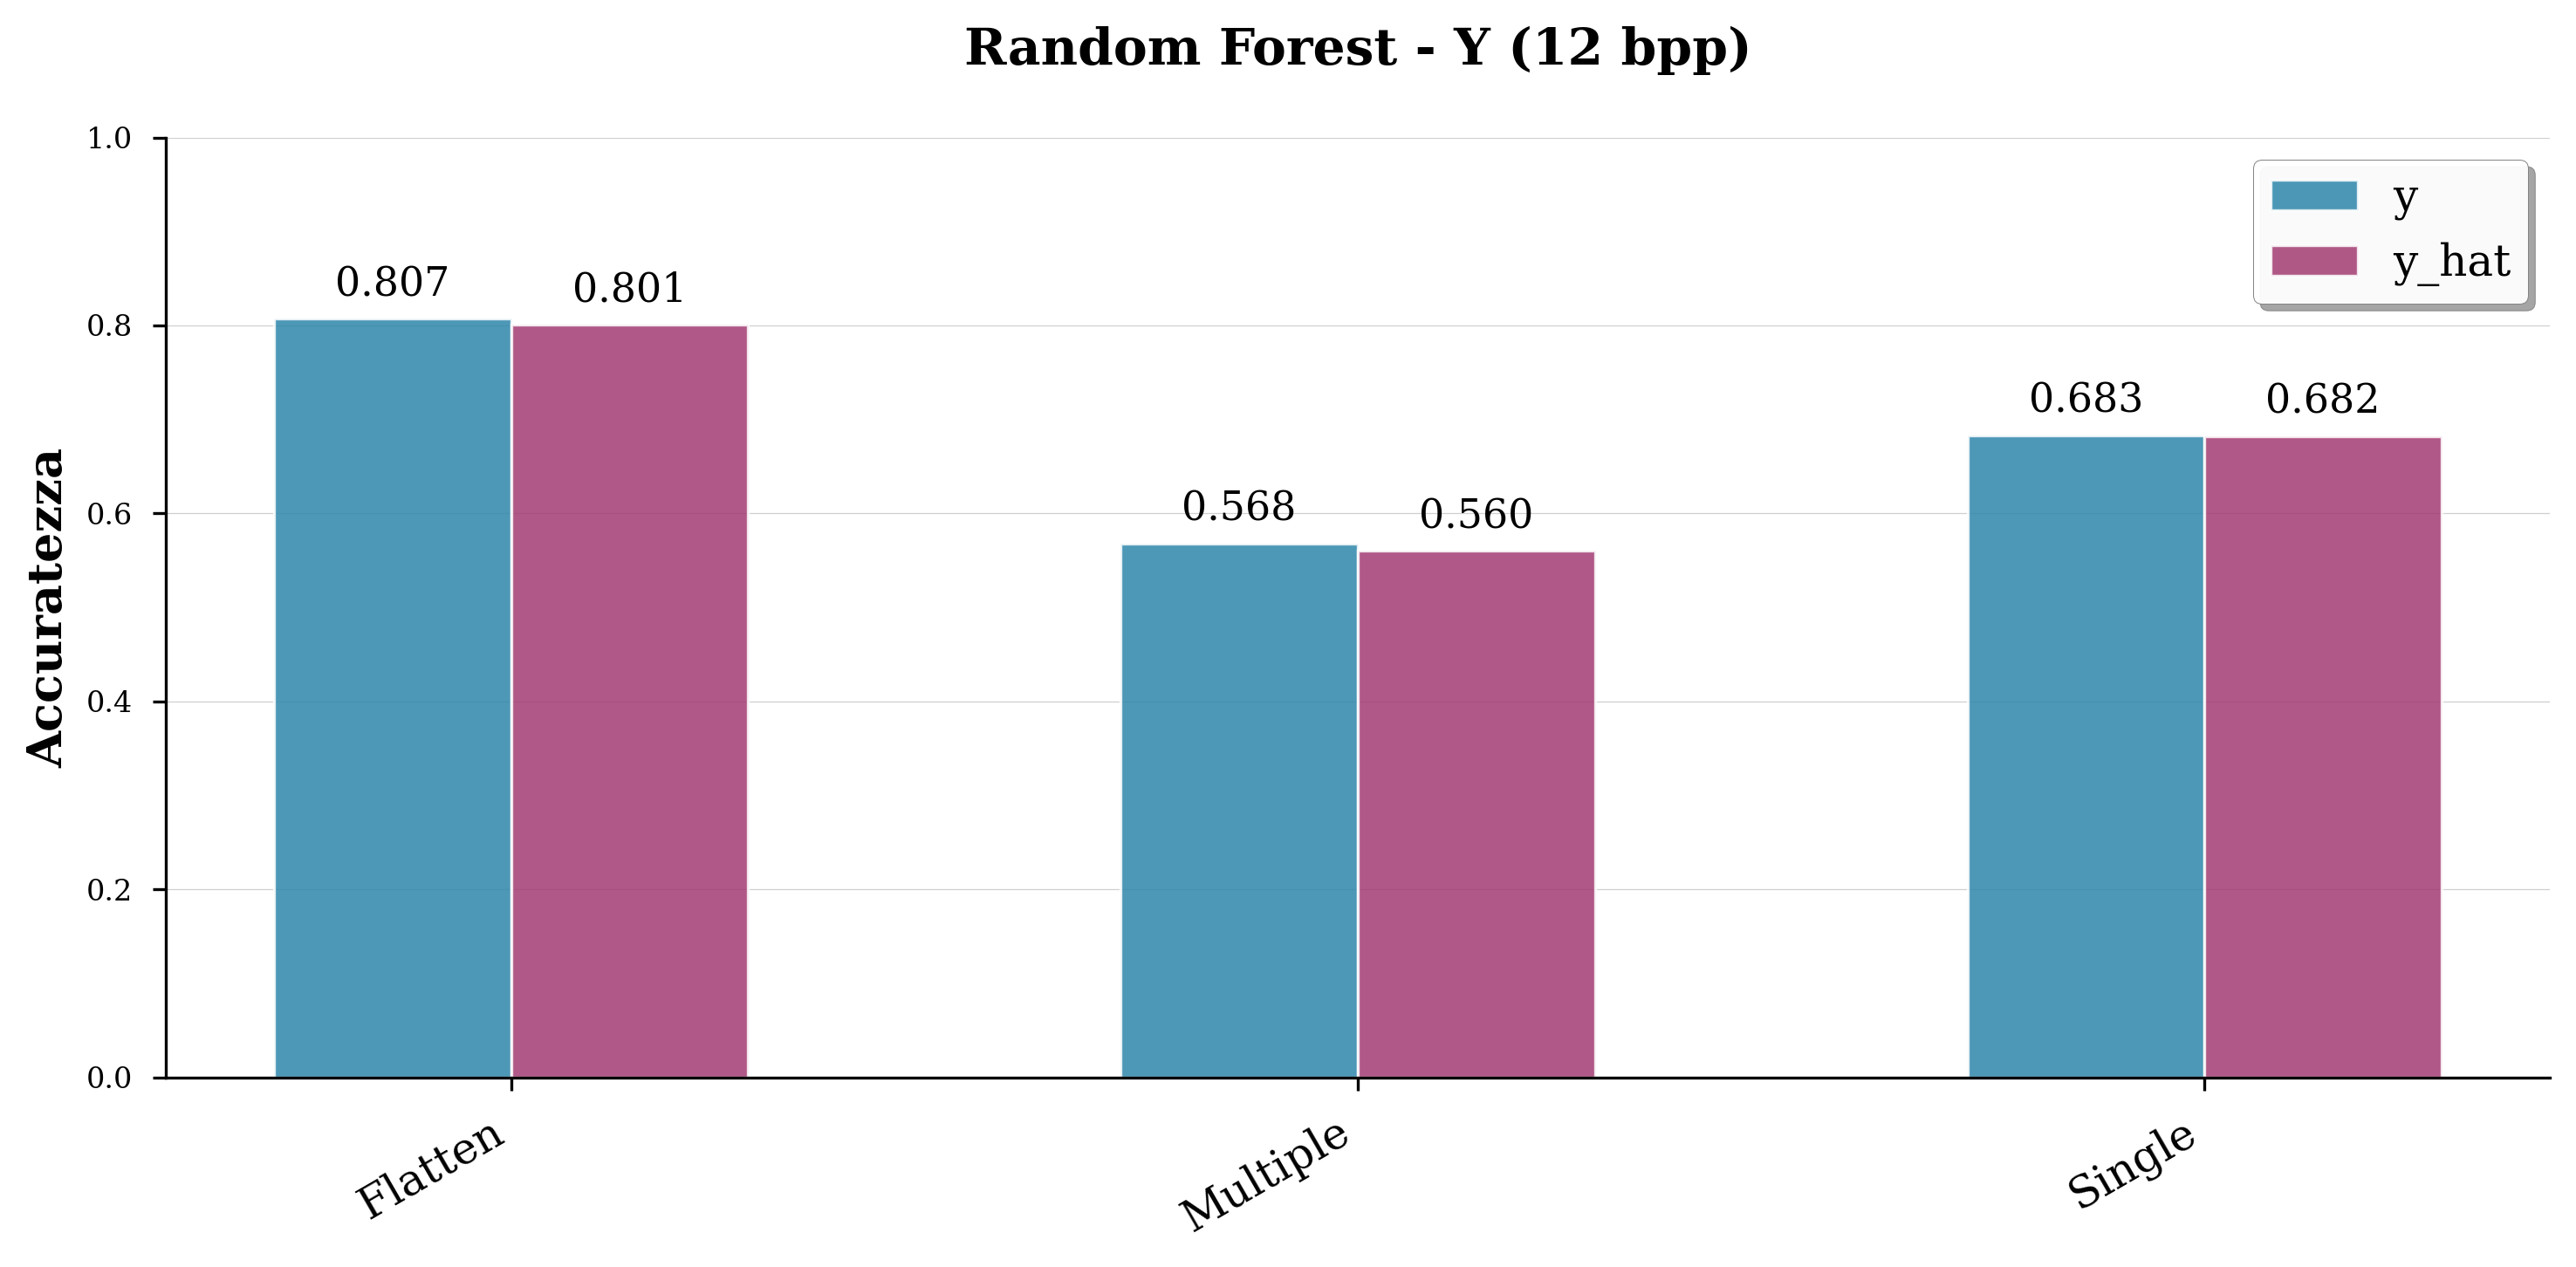
\includegraphics[width=\textwidth]{figures/RF_Y_12bpp_improved.png}\\[0.5cm]
    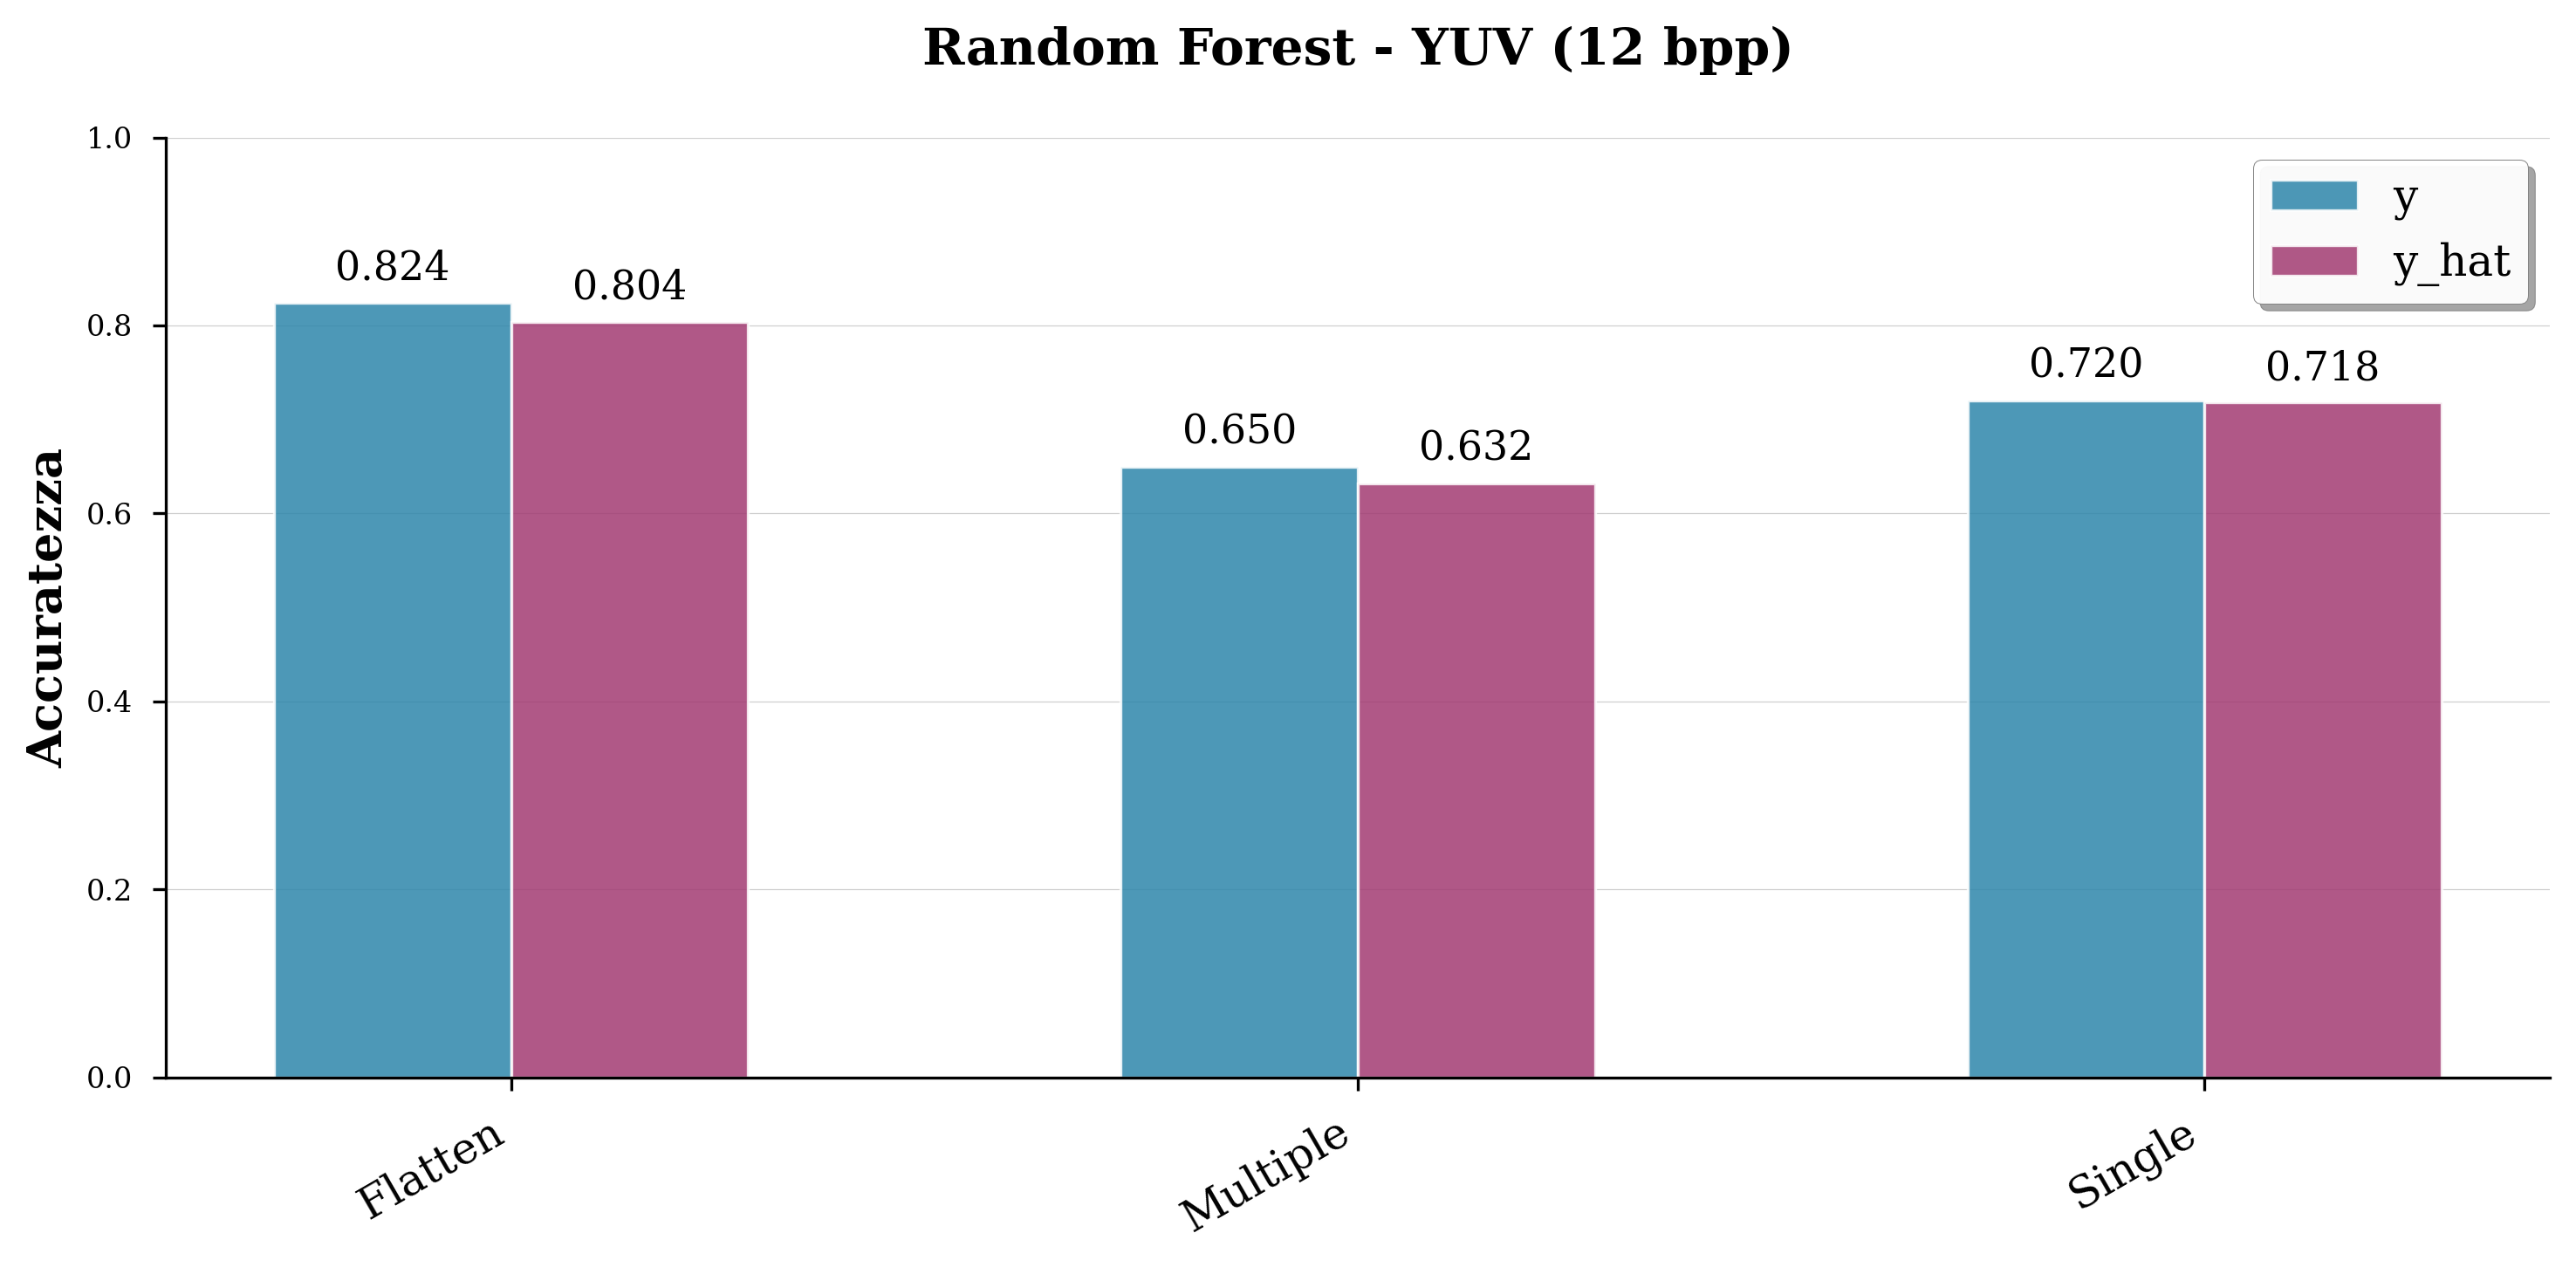
\includegraphics[width=\textwidth]{figures/RF_YUV_12bpp_improved.png}
    \caption{Confronto tra prestazioni di due Random Forest allenati Y e YUV.}
    \label{fig:RF_YvsYUV}
\end{figure}
\\
Nella figura \ref{fig:RF_YvsYUV} si nota come le prestazioni del Random Forest allenato su YUV siano  migliori rispetto a quello allenato esclusivamente su Y, in particolare nel caso del metodo di processing "single patch"; questo comportamento rispetta le aspettative descritte nella sez. \ref{subsec:choices}. Si può anche notare come nella maggior parte degli esperimenti, i modelli allenati sulle rappresentazioni non quantizzate ottengano risultati migliori rispetto a quelli allenati sulle rappresentazioni quantizzate.

Nella figura \ref{fig:RF_YUV_confusion} sono riportate le matrici di confusione per le configurazioni che hanno ottenuto migliori prestazioni con l'uso di Random Forest.
\begin{figure}[H]
    \centering
    \begin{subfigure}[b]{0.8\textwidth}
        \centering
        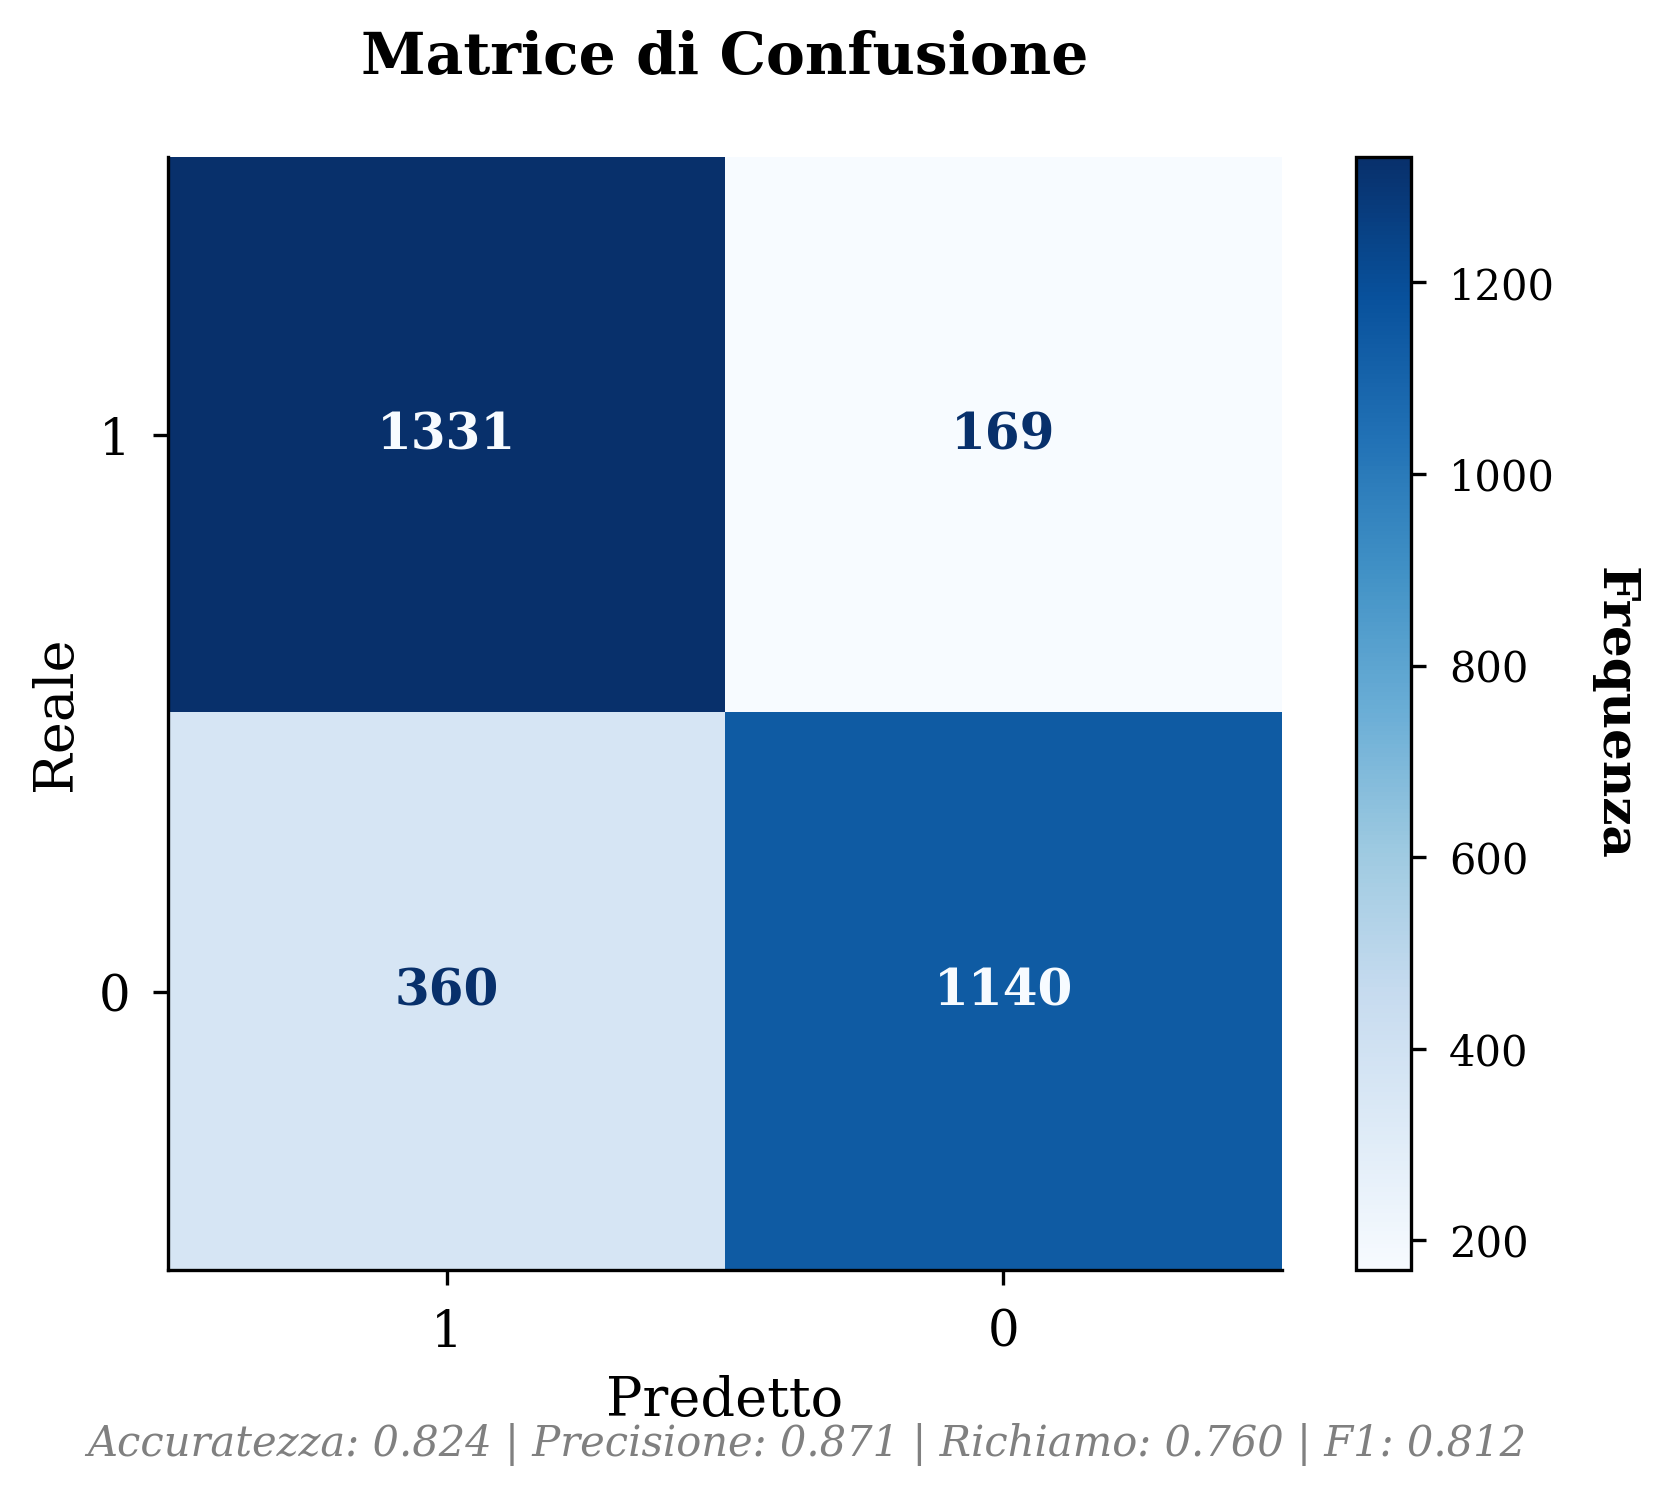
\includegraphics[width=\textwidth]{figures/confusion_matrix_flatten_YUV_RF.png}
        \caption{Metodo flatten}
    \end{subfigure}
    \hfill
    \begin{subfigure}[b]{0.8\textwidth}
        \centering
        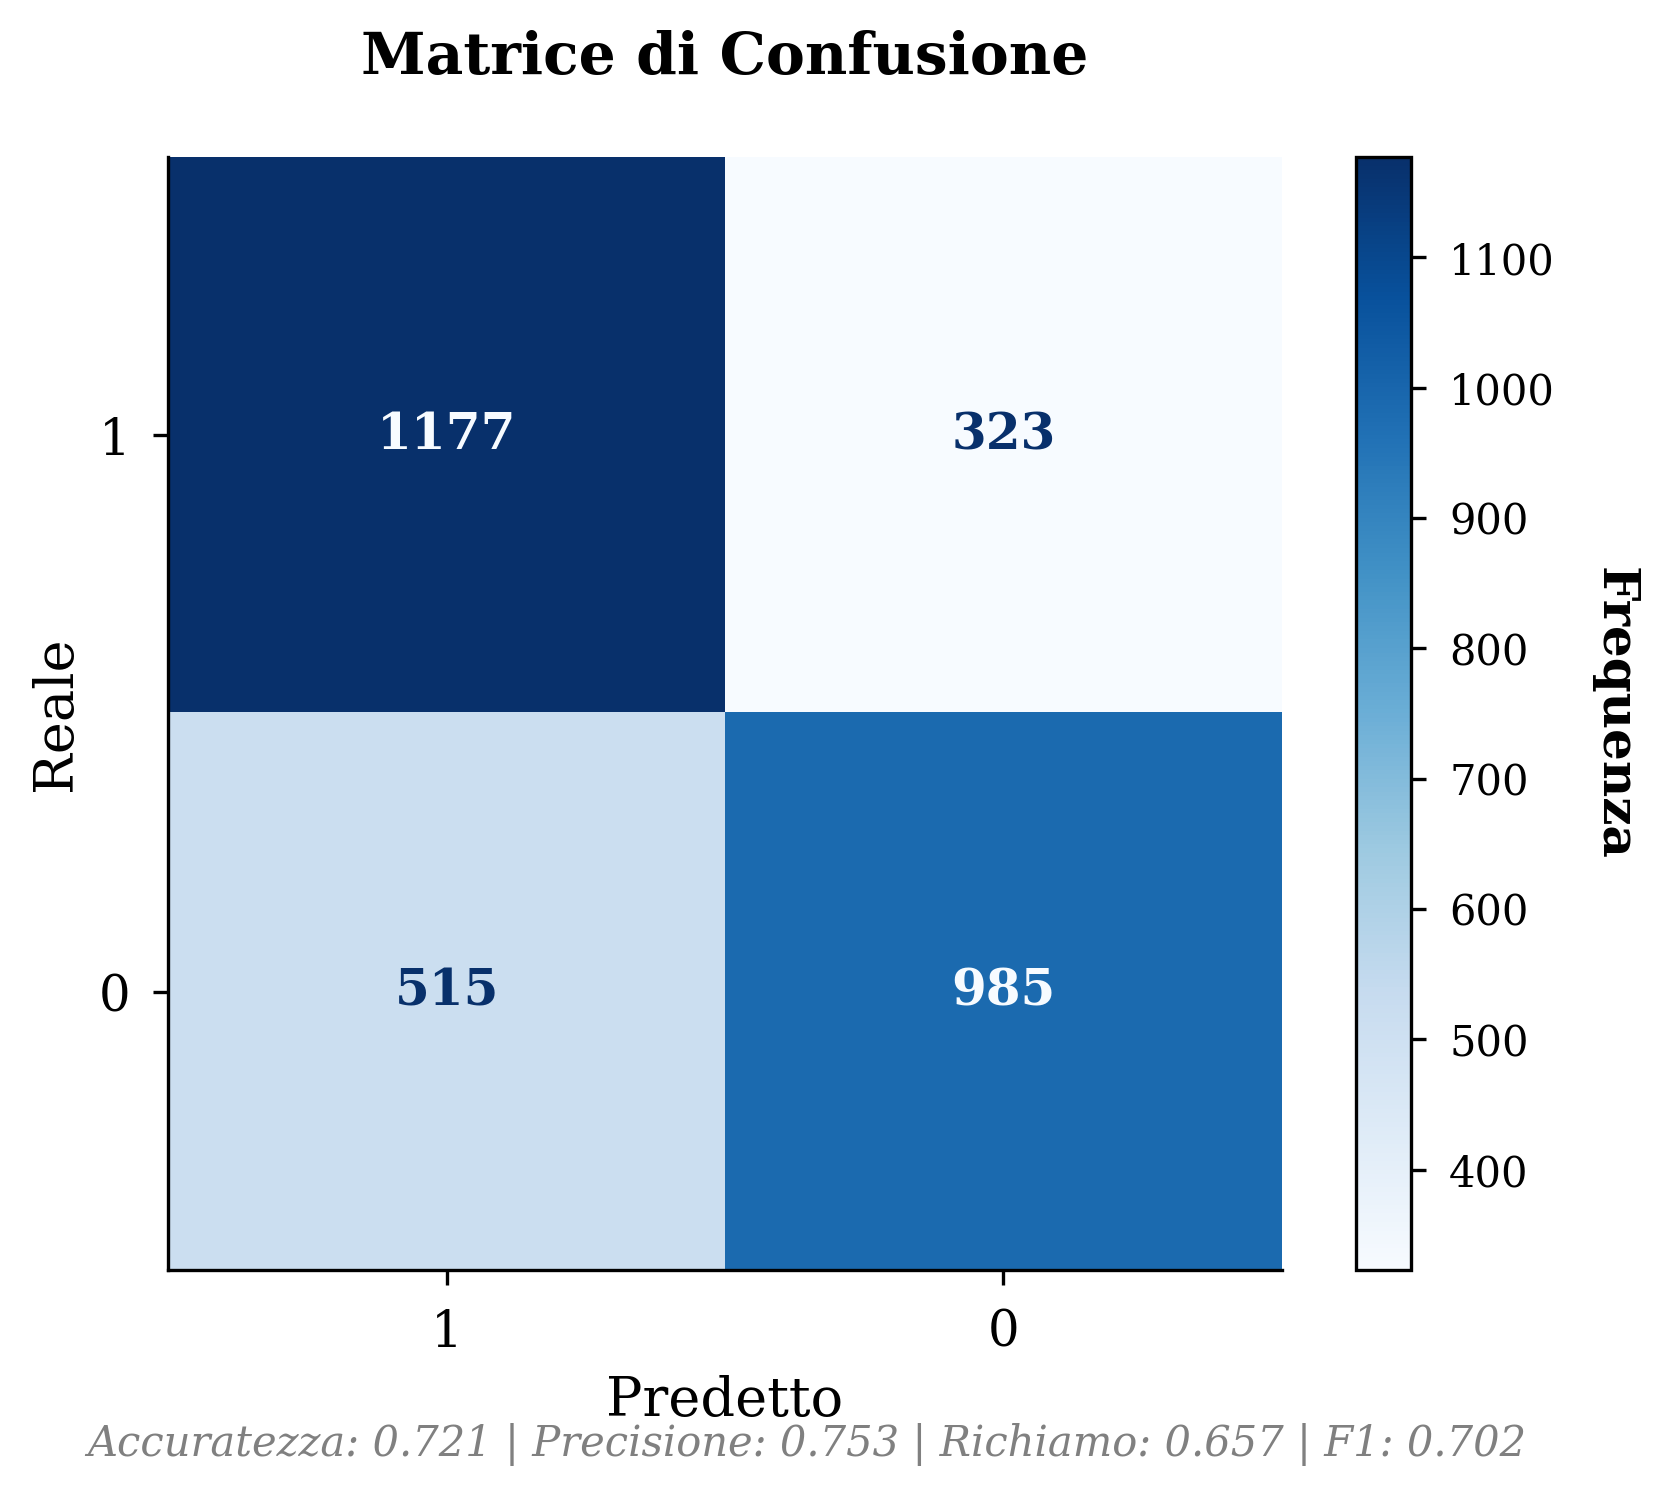
\includegraphics[width=\textwidth]{figures/confusion_matrix_YUV_single_RF.png}
        \caption{Metodo single patch}
    \end{subfigure}
    \caption{Matrici di confusione per Random Forest allenato usando YUV e processando le feature con (a) flatten e (b) single patch.}
    \label{fig:RF_YUV_confusion}
\end{figure}

\subsection{GradientBoosting}
Con la ricerca dei parametri ottimali, la combinazione migliore di iperparametri trovata per l'algoritmo di Gradient Boosting è:
\begin{lstlisting}[style=pythonElegant]
    GradientBoostingClassifier(
        learning_rate=0.12965912630431367, 
        max_iter=596, 
        max_leaf_nodes=117,
        min_samples_leaf=18, 
        l2_regularization=0.003042734607209594,
        random_state=42, validation_fraction=0.1)
\end{lstlisting}
Come fatto per il Random Forest, nella tabella \ref{tab:GB-results-table} sono riportati tutti i risultati ottenuti da Gradient Boosting.
\begin{table}[H]
\centering
\caption{Risultati per Gradient Boosting}
\label{tab:GB-results-table}
\begin{tabular}{lrllrr}
\toprule
Modello &  Bpp &  Comp. &     process. &     y &  y\_hat \\
\midrule
GB &  6 &       Y &   single & 0.696 &  0.688 \\
GB &  6 &       Y & multiple & 0.543 &  0.535 \\
GB &  6 &       Y & flatten & 0.890 & 0.870 \\
GB & 12 &       Y &   single & 0.695 &  0.700 \\
GB & 12 &       Y & multiple & 0.554 &  0.534 \\
GB & 12 &       Y & flatten & 0.900 & 0.890 \\
\midrule
GB &  6 &     YUV &   single & 0.744 &  0.753 \\
GB &  6 &     YUV & multiple & 0.670 &  0.645 \\
GB &  6 &     YUV &  flatten & 0.940 &  0.940 \\
GB & 12 &     YUV &   single & 0.744 &  0.744 \\
GB & 12 &     YUV & multiple & 0.680 &  0.667 \\
GB & 12 &     YUV &  flatten & 0.944 &  0.940 \\
\bottomrule
\end{tabular}
\end{table}
\begin{figure}[H]
    \centering
    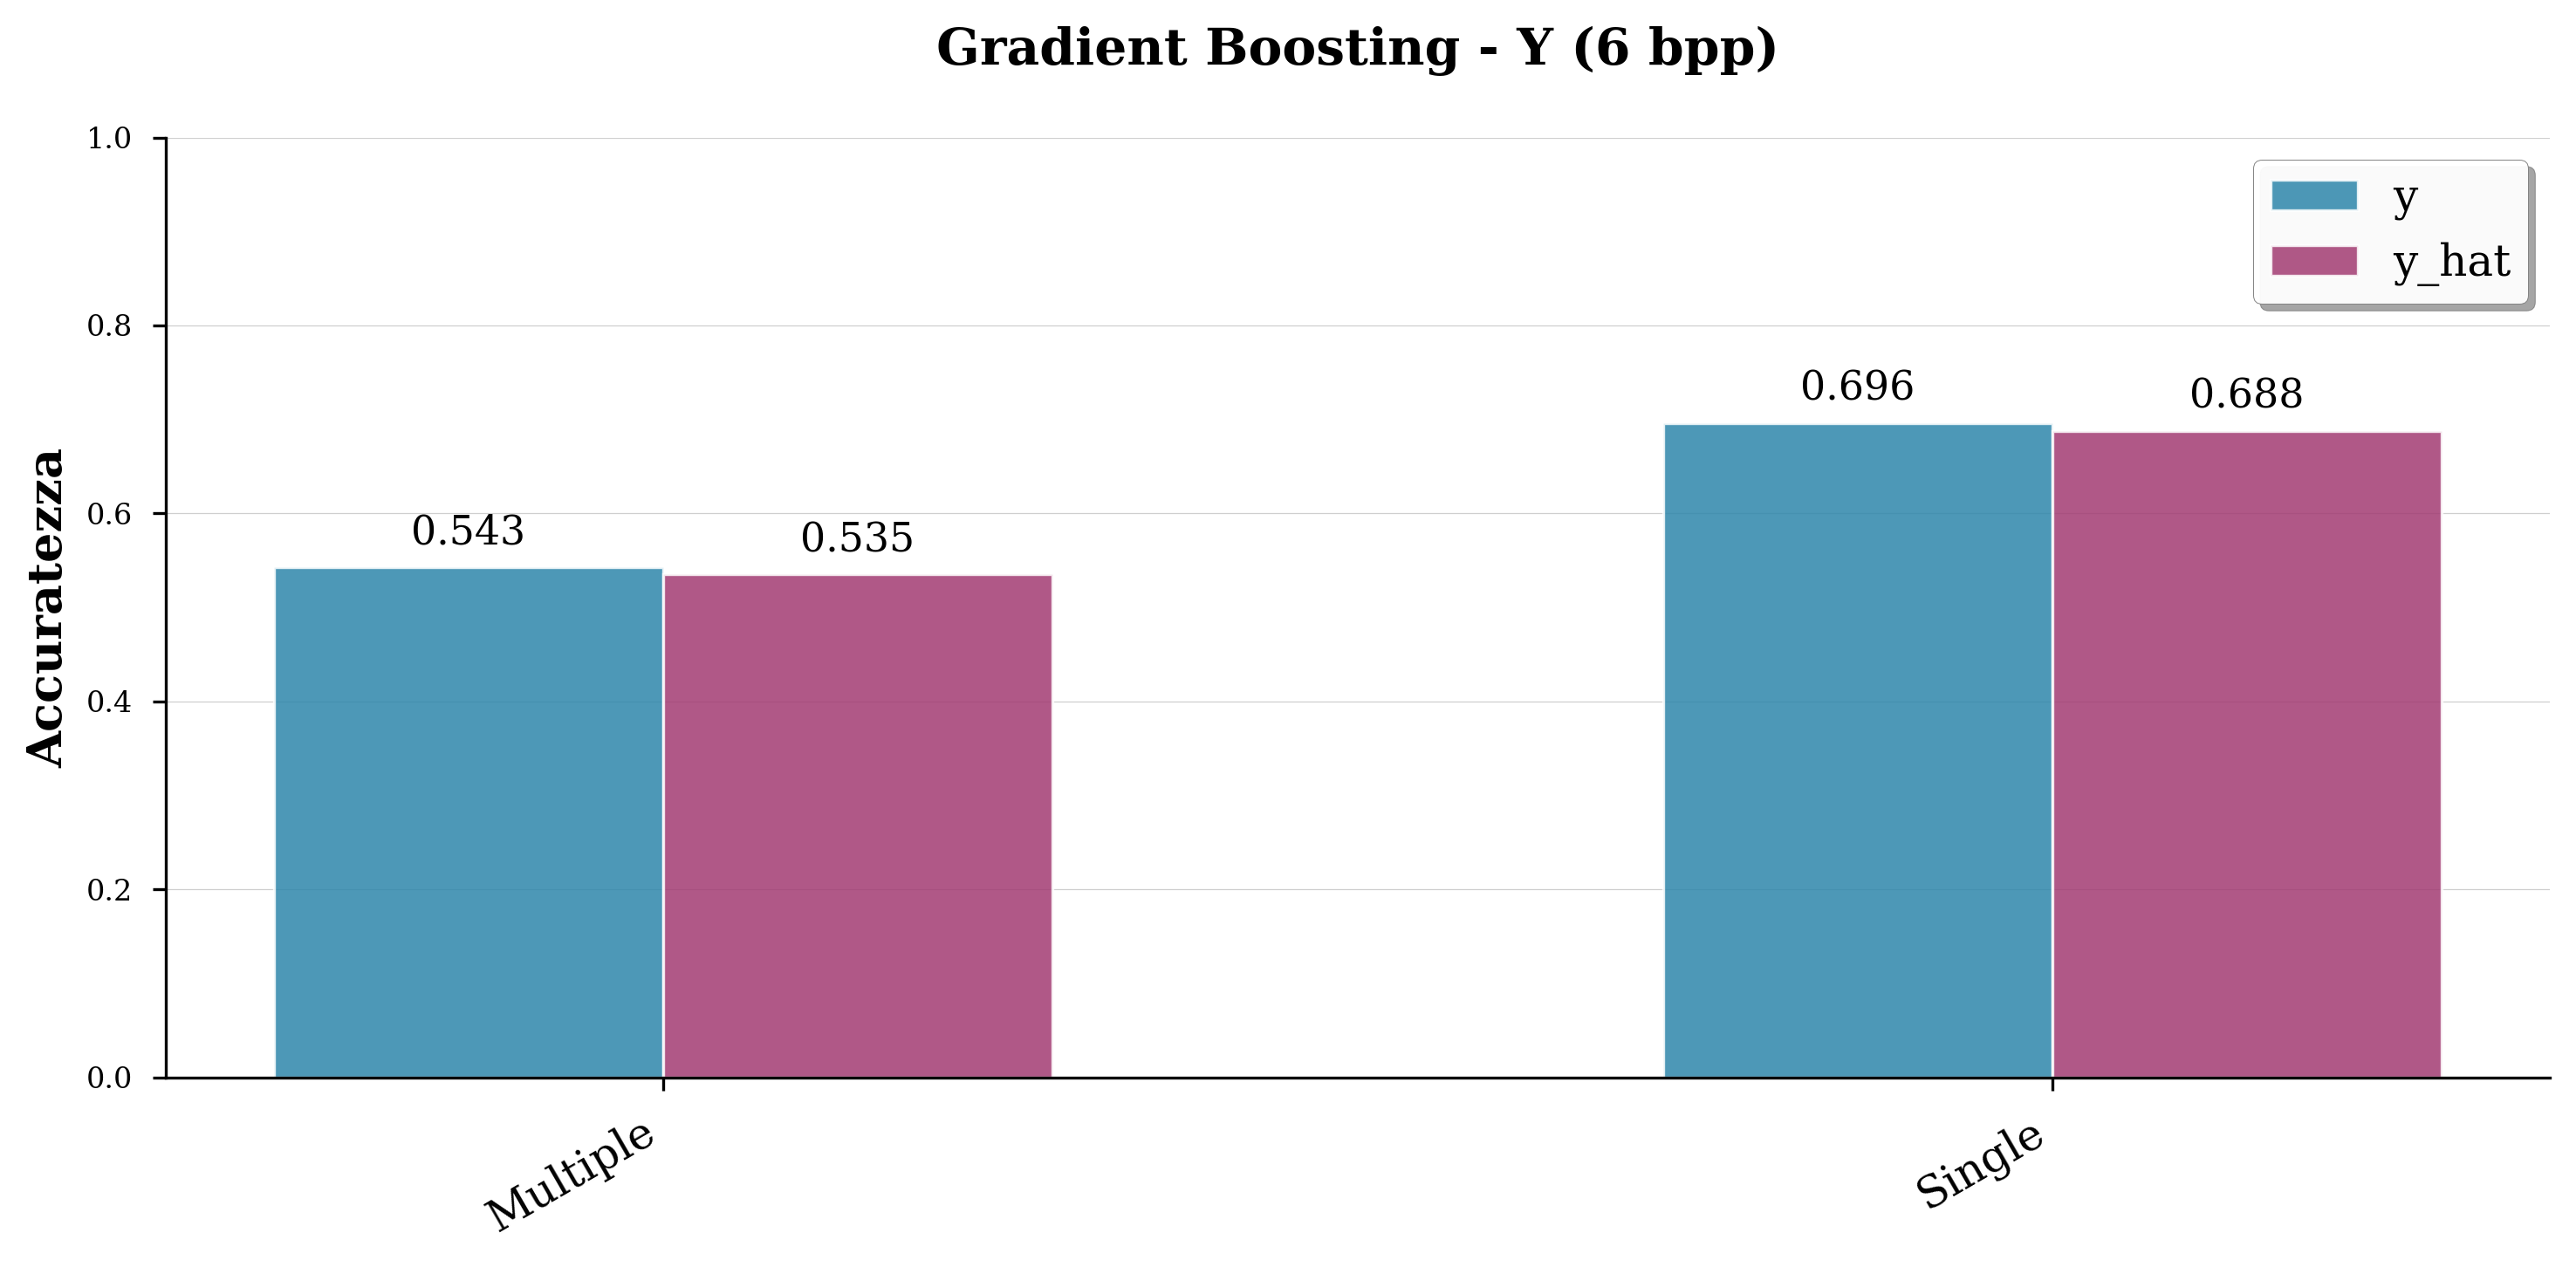
\includegraphics[width=\textwidth]{figures/GB_Y_6bpp_improved.png}\\[0.5cm]
    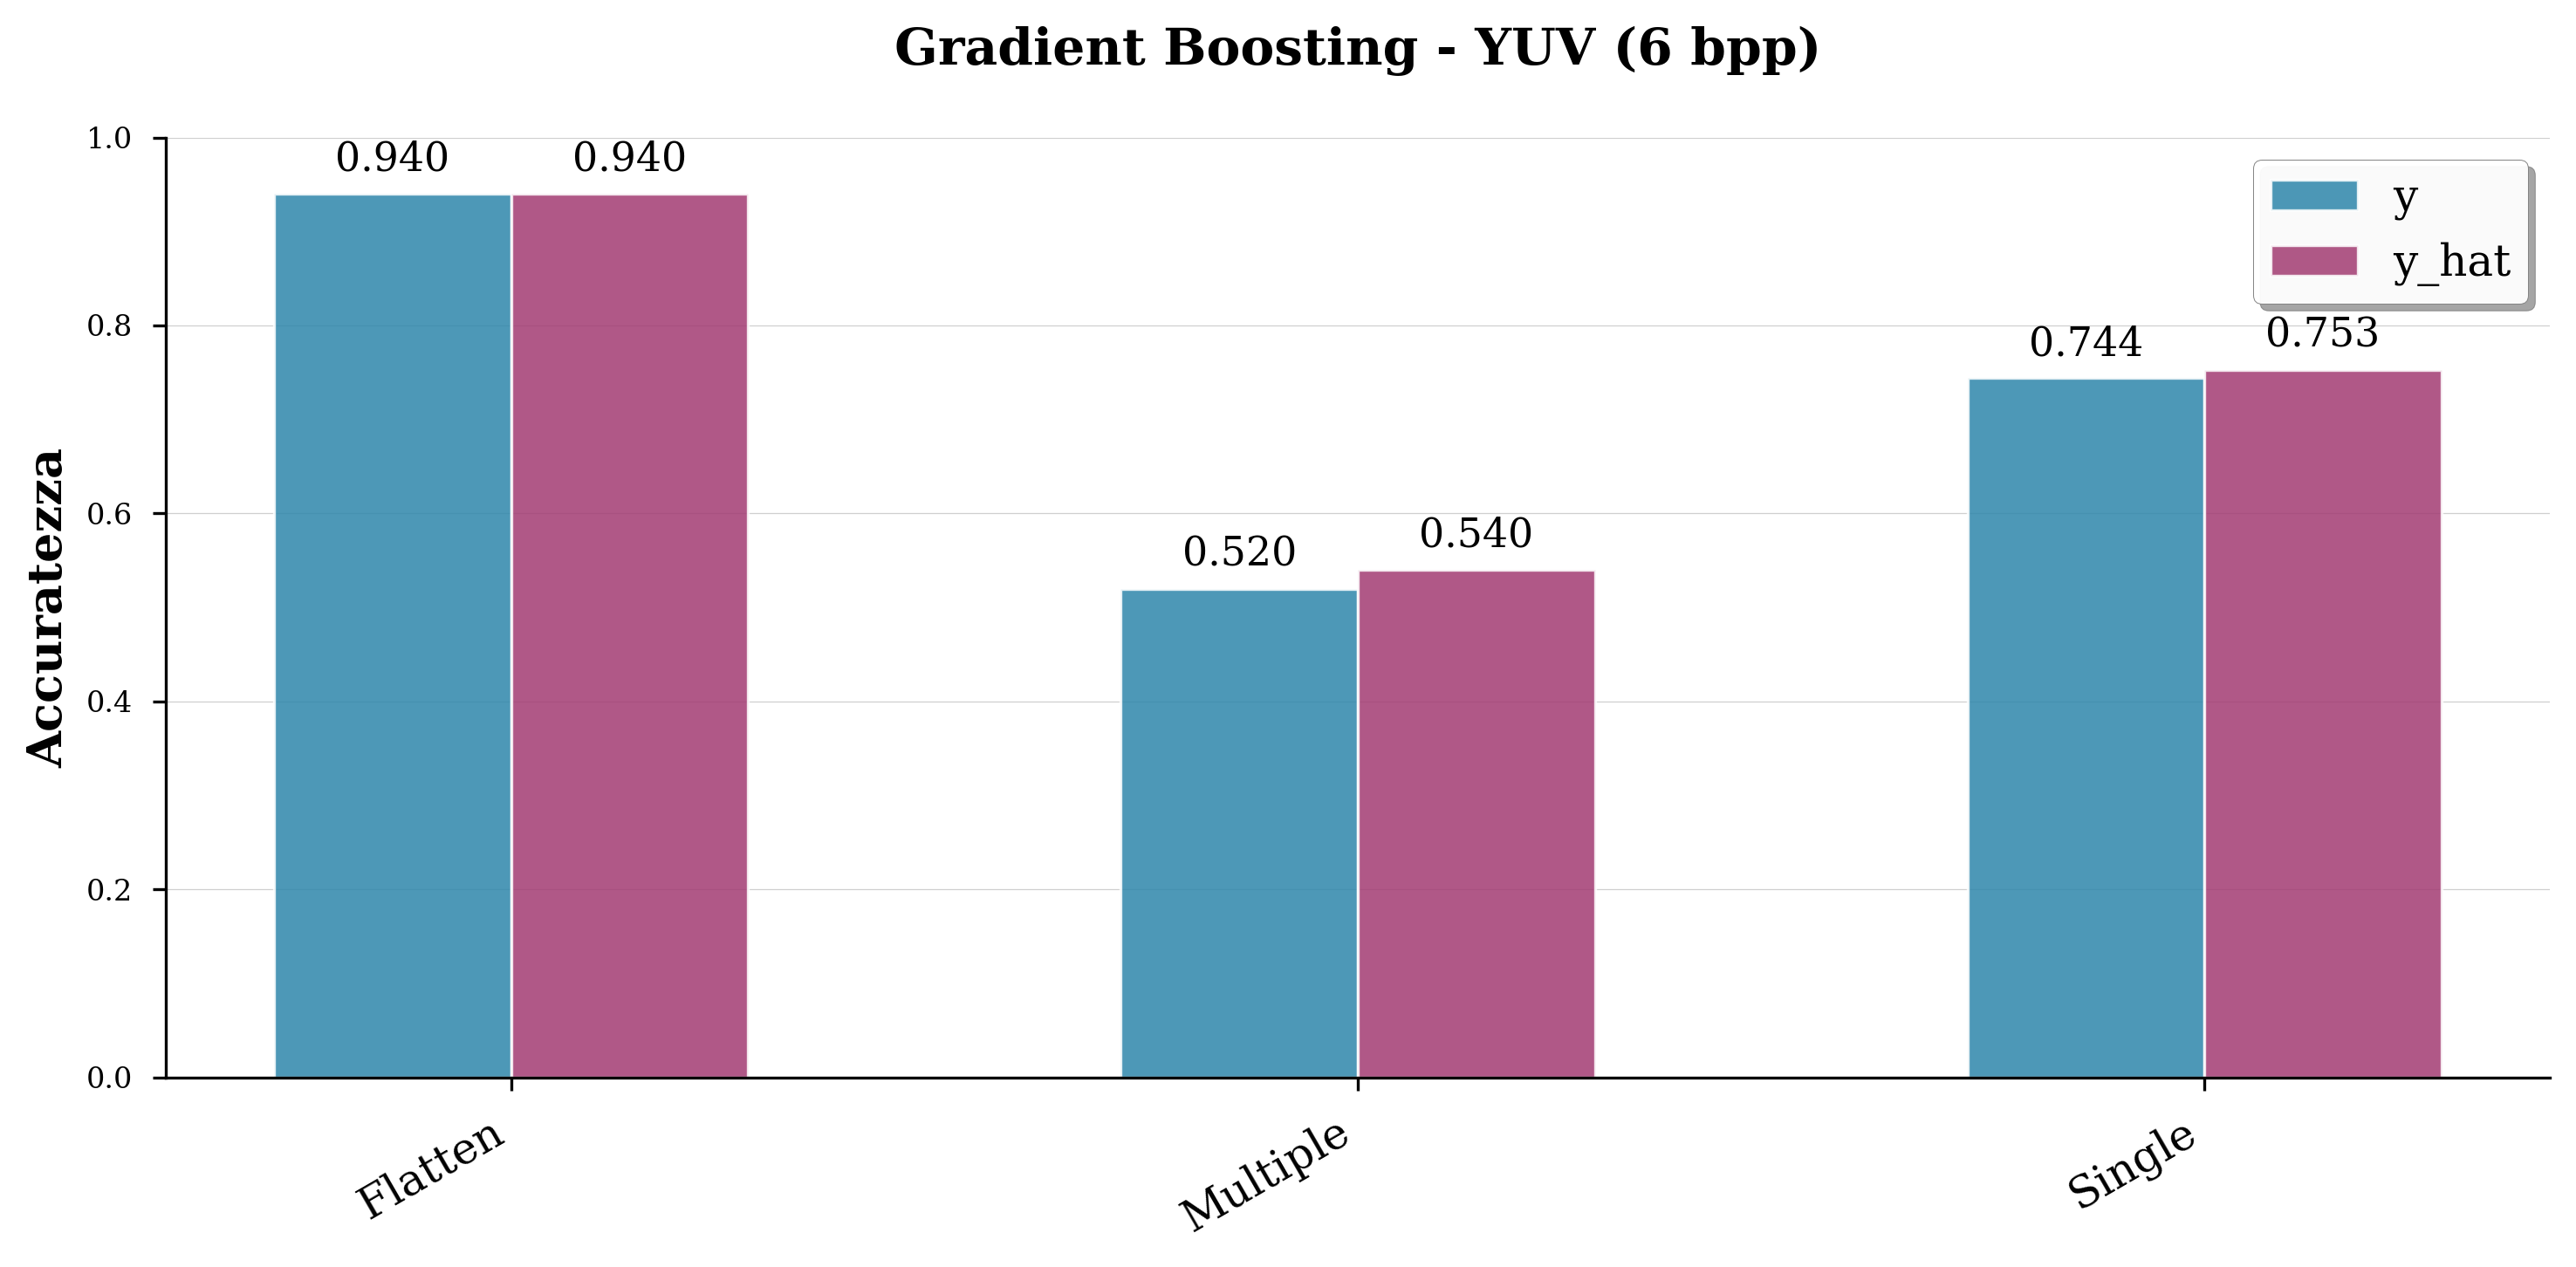
\includegraphics[width=\textwidth]{figures/GB_YUV_6bpp_improved.png}
    \caption{Esempi di diagrammi a barre riguardanti performance di Gradient Boosting}
    \label{fig:GB_YUV_plots}
\end{figure}
Dai risultati ottenuti si nota un comportamento simile a quello del Random Forest, ottenendo migliori prestazioni con il metodo flatten e l'uso di tutte e tre le componenti YUV.
Nella figura \ref{fig:GB_YUV_confusion} sono riportate le matrici di confusione per le configurazioni che hanno ottenuto migliori prestazioni.
\begin{figure}[H]
    \centering
    \begin{subfigure}[b]{0.7\textwidth}
        \centering
        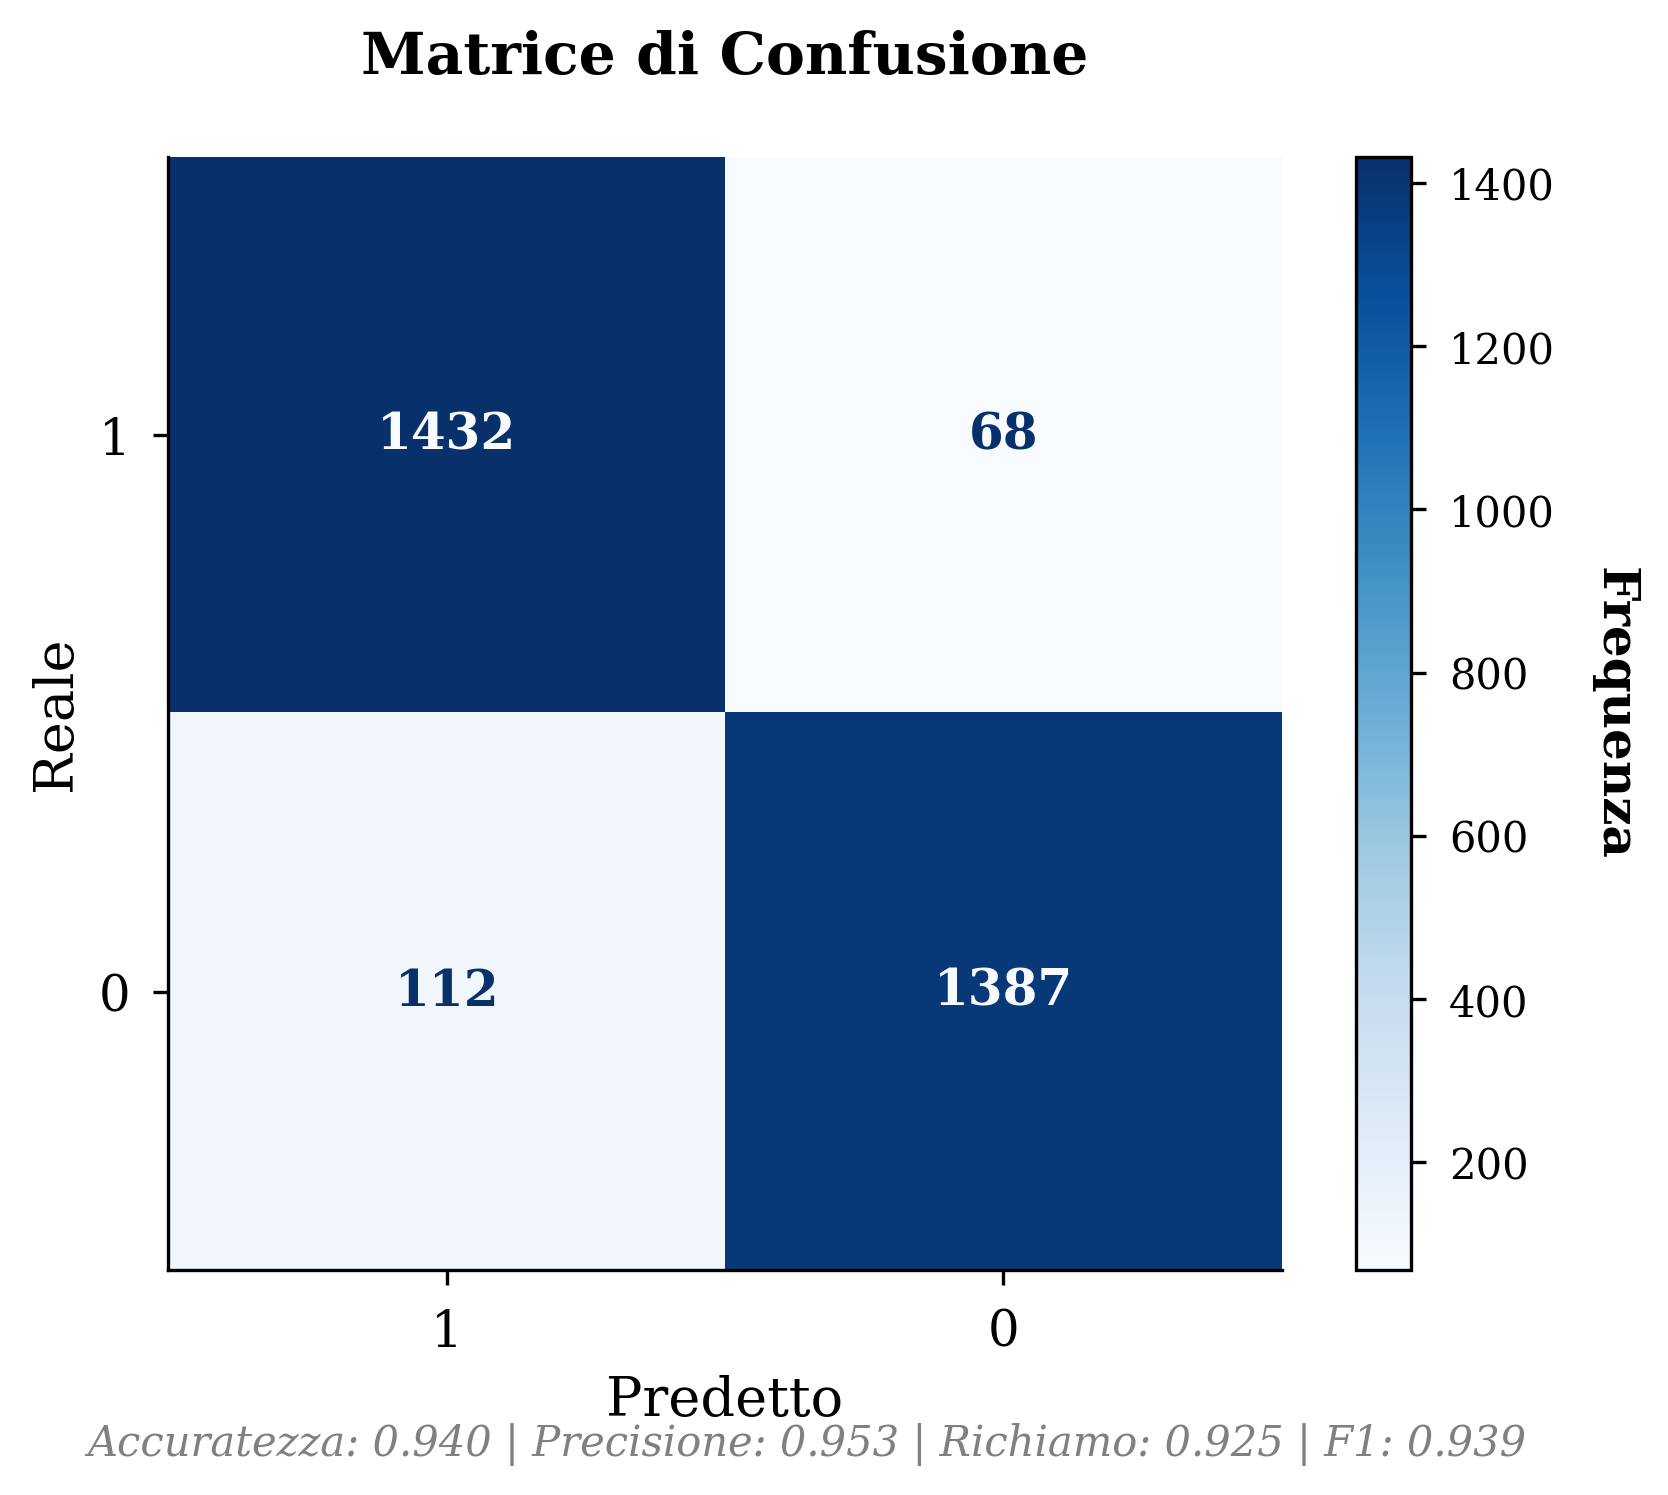
\includegraphics[width=\textwidth]{figures/confusion_matrix_YUV_flatten_GB.png}
        \caption{Metodo flatten}
    \end{subfigure}
    \hfill
    \begin{subfigure}[b]{0.7\textwidth}
        \centering
        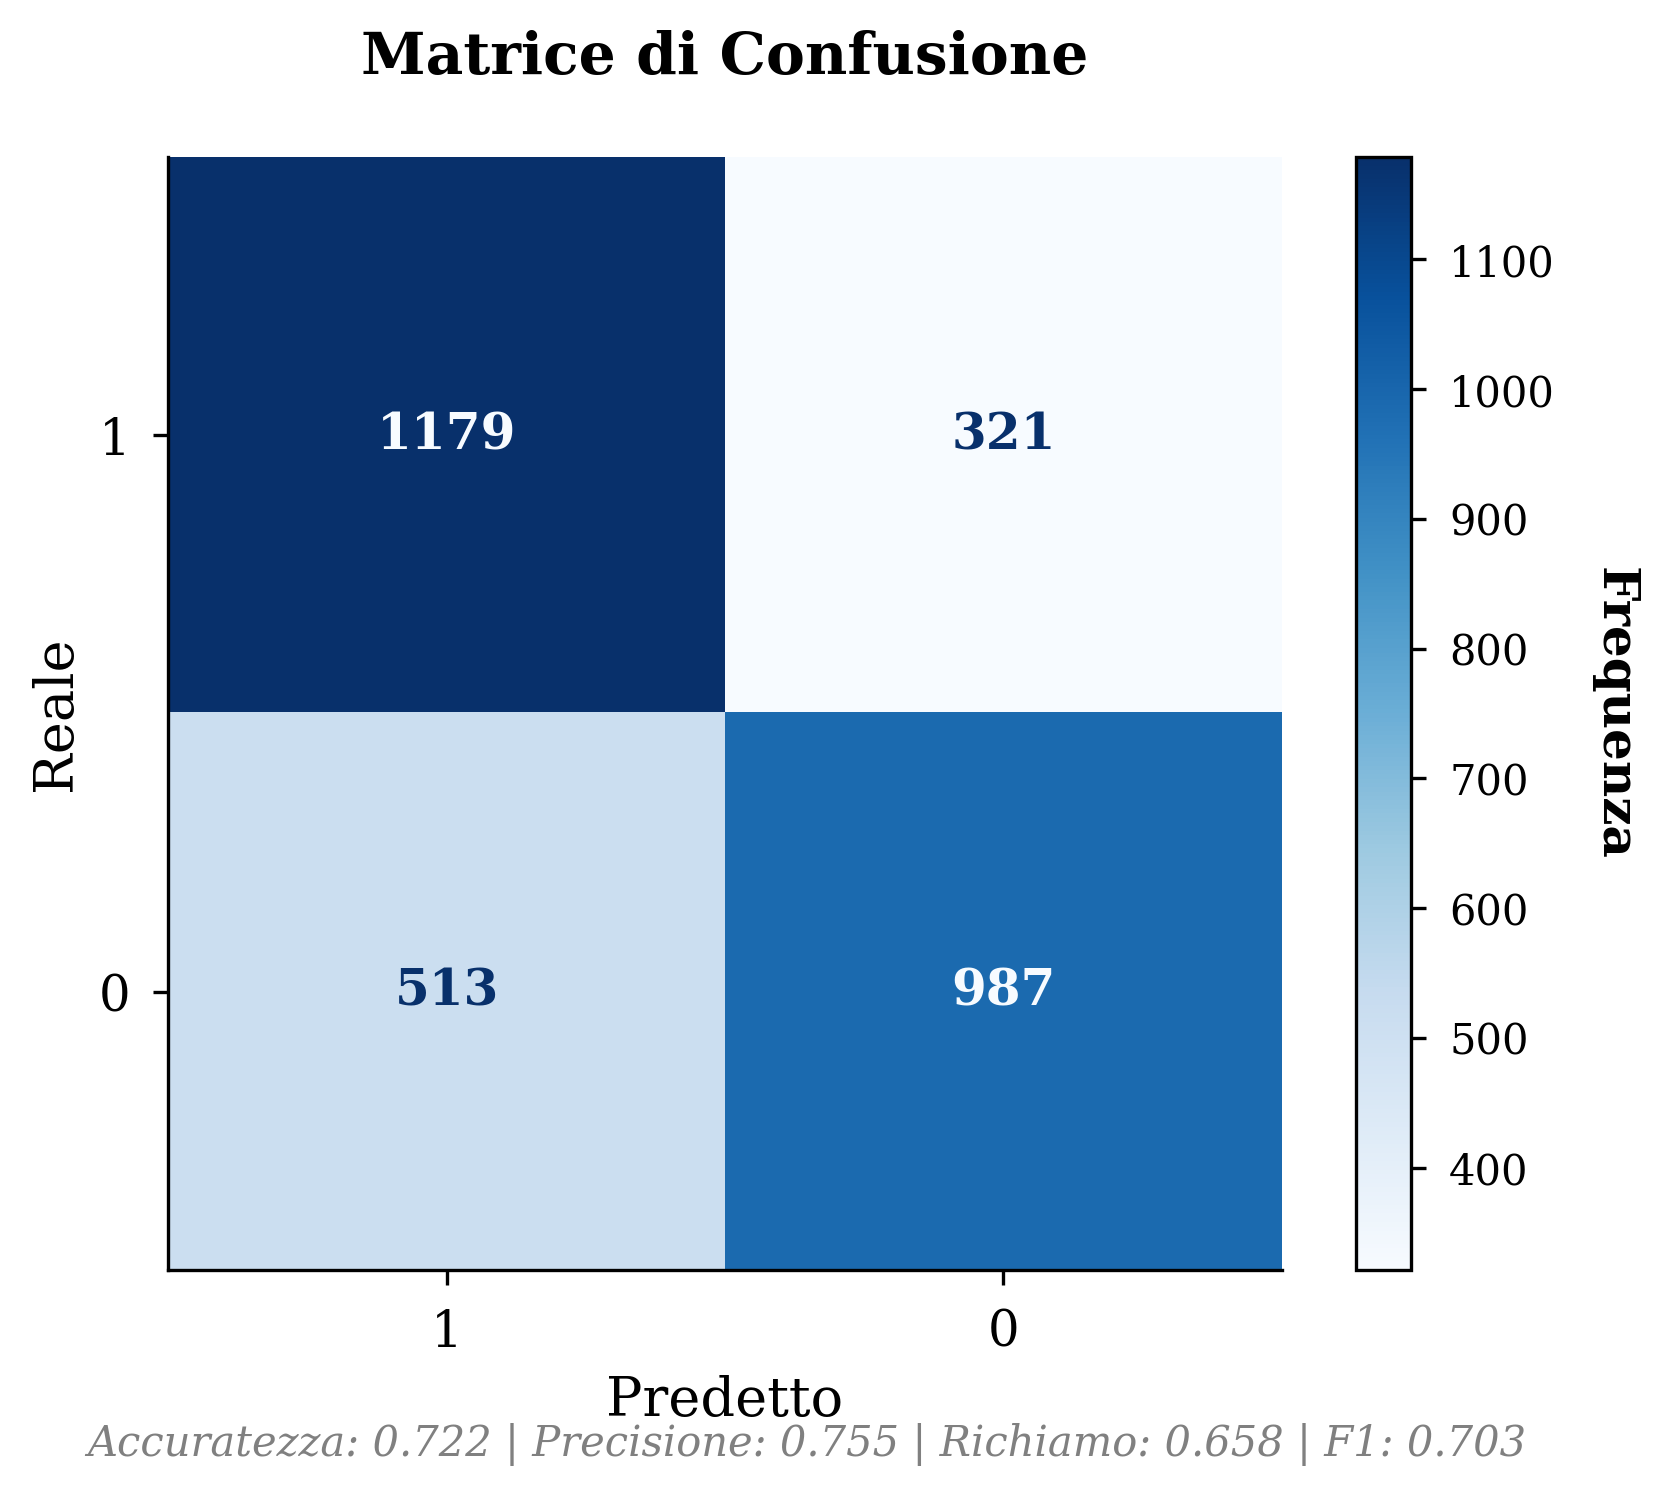
\includegraphics[width=\textwidth]{figures/confusion_matrix_YUV_single_GB.png}
        \caption{Metodo single patch}
    \end{subfigure}
    \caption{Matrici di confusione per Gradient Boosting allenato su YUV con due approcci diversi.}
    \label{fig:GB_YUV_confusion}
\end{figure}
\section{Analisi dei risultati}
Nei diagrammi presenti nelle figure \ref{fig:GB_RF_Y_comparison} e \ref{fig:GB_RF_YUV_comparison} viene mostrato il confronto diretto tra le prestazioni dei due classificatori a diversi in tutte le configurazioni testate.
\begin{figure}
    \centering
    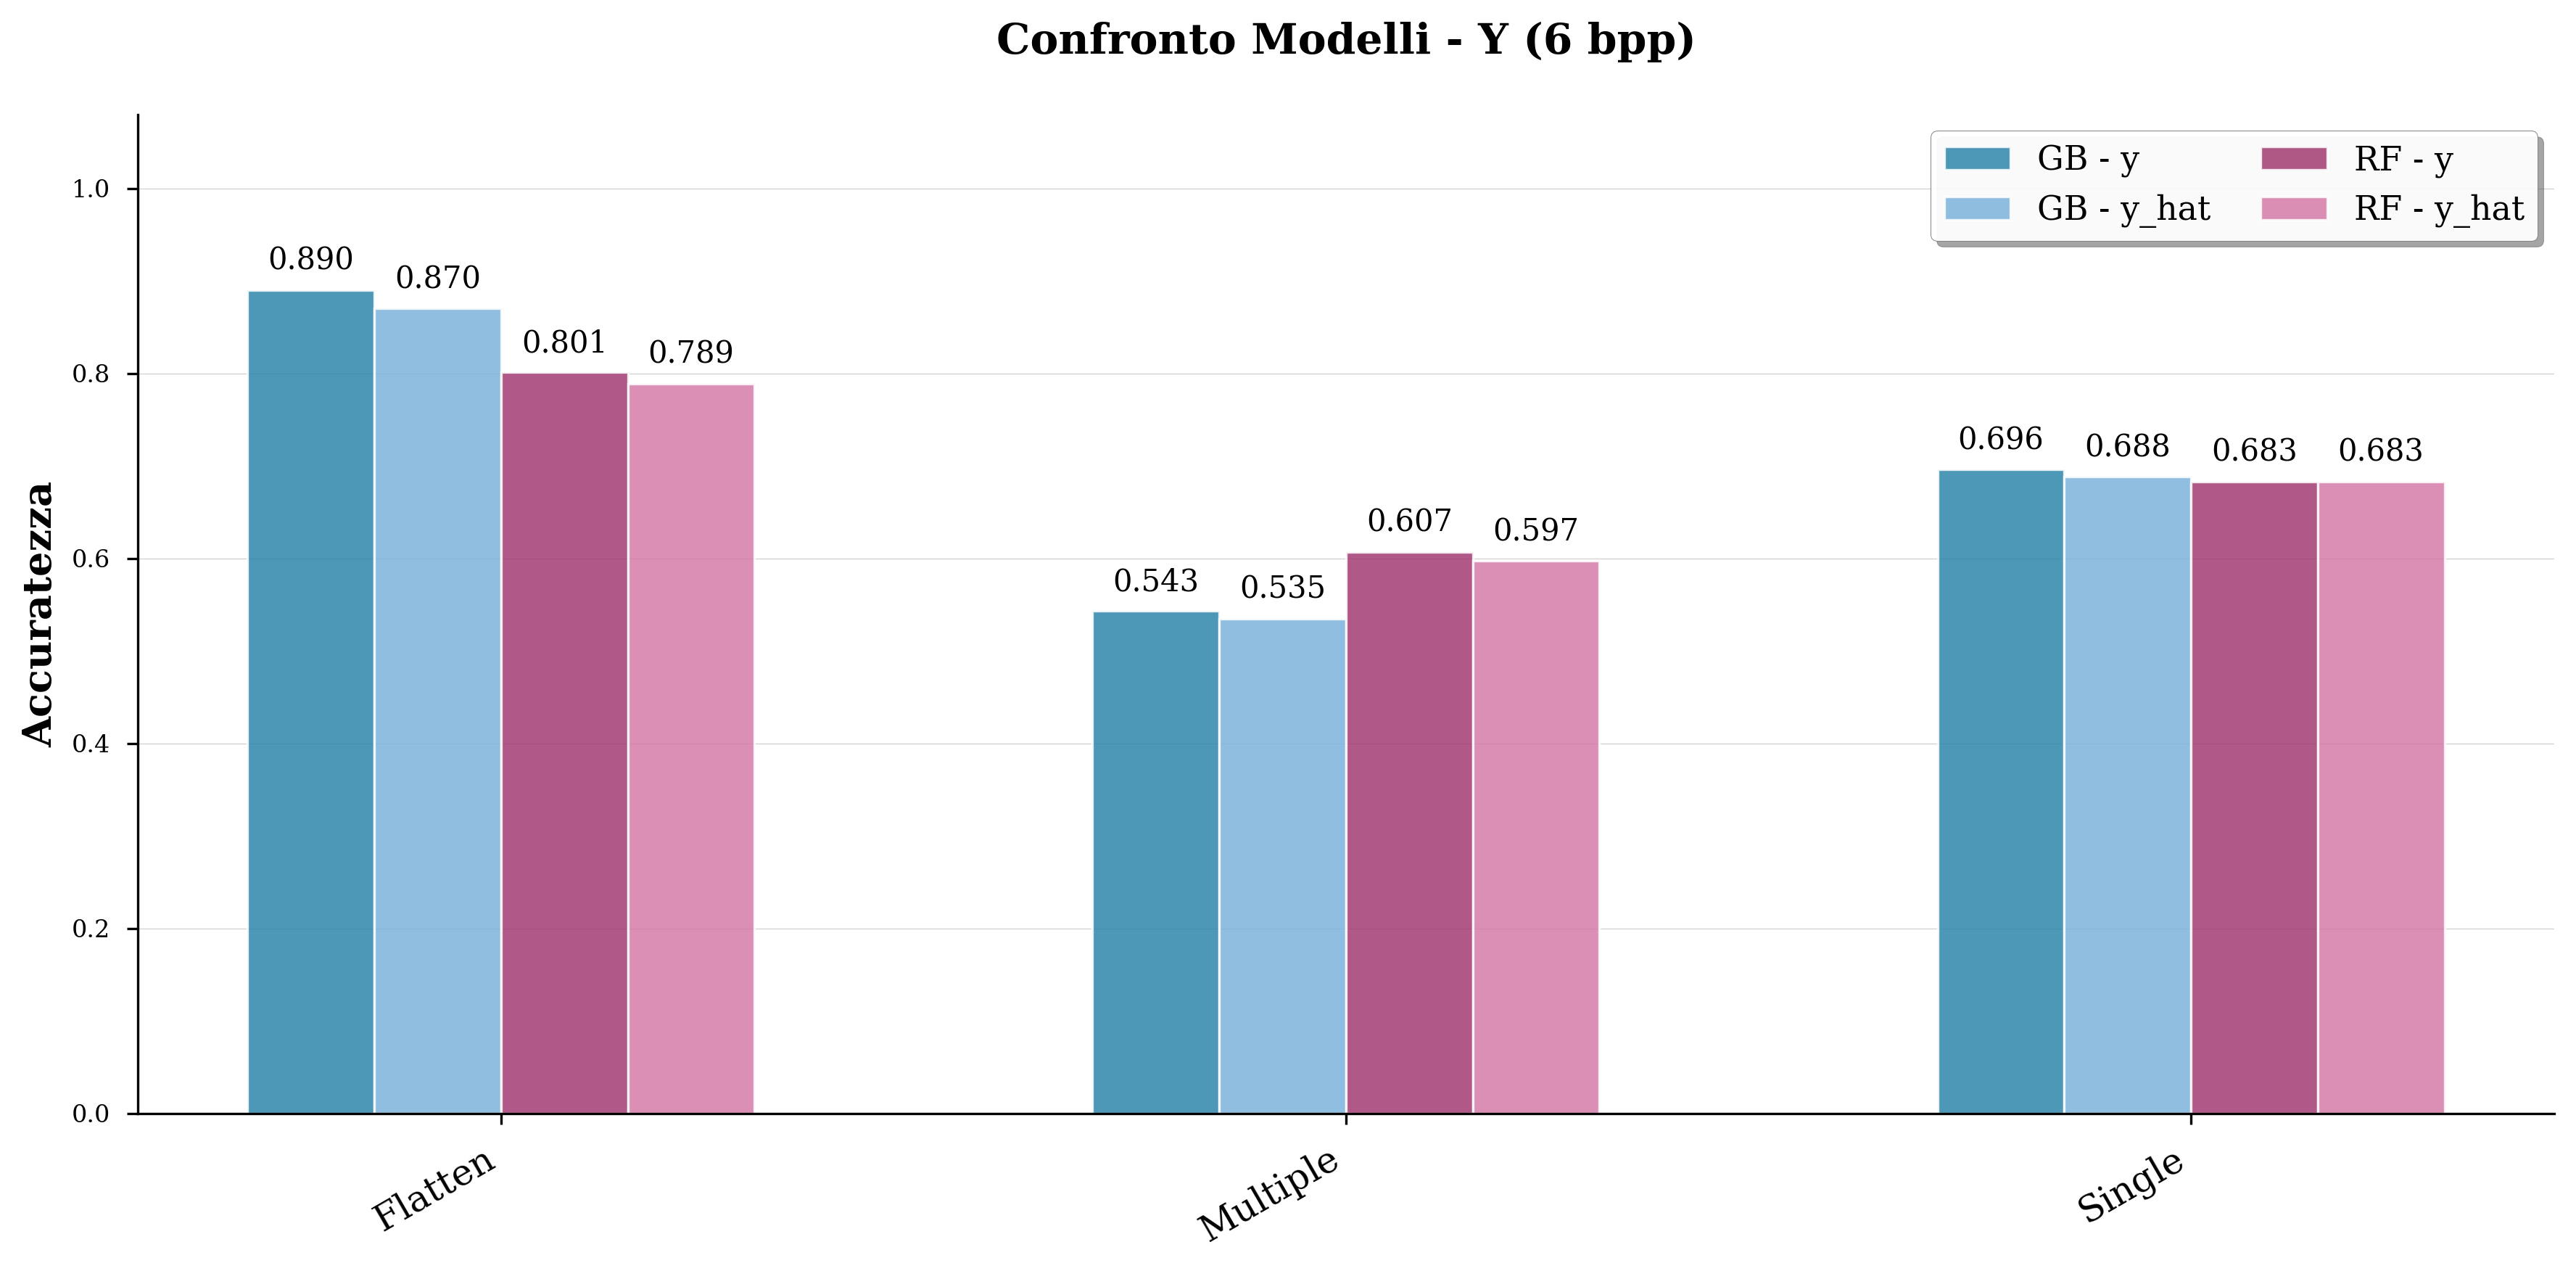
\includegraphics[width=\textwidth]{figures/Compare_GB_RF_Y_6bpp_improved.png}
    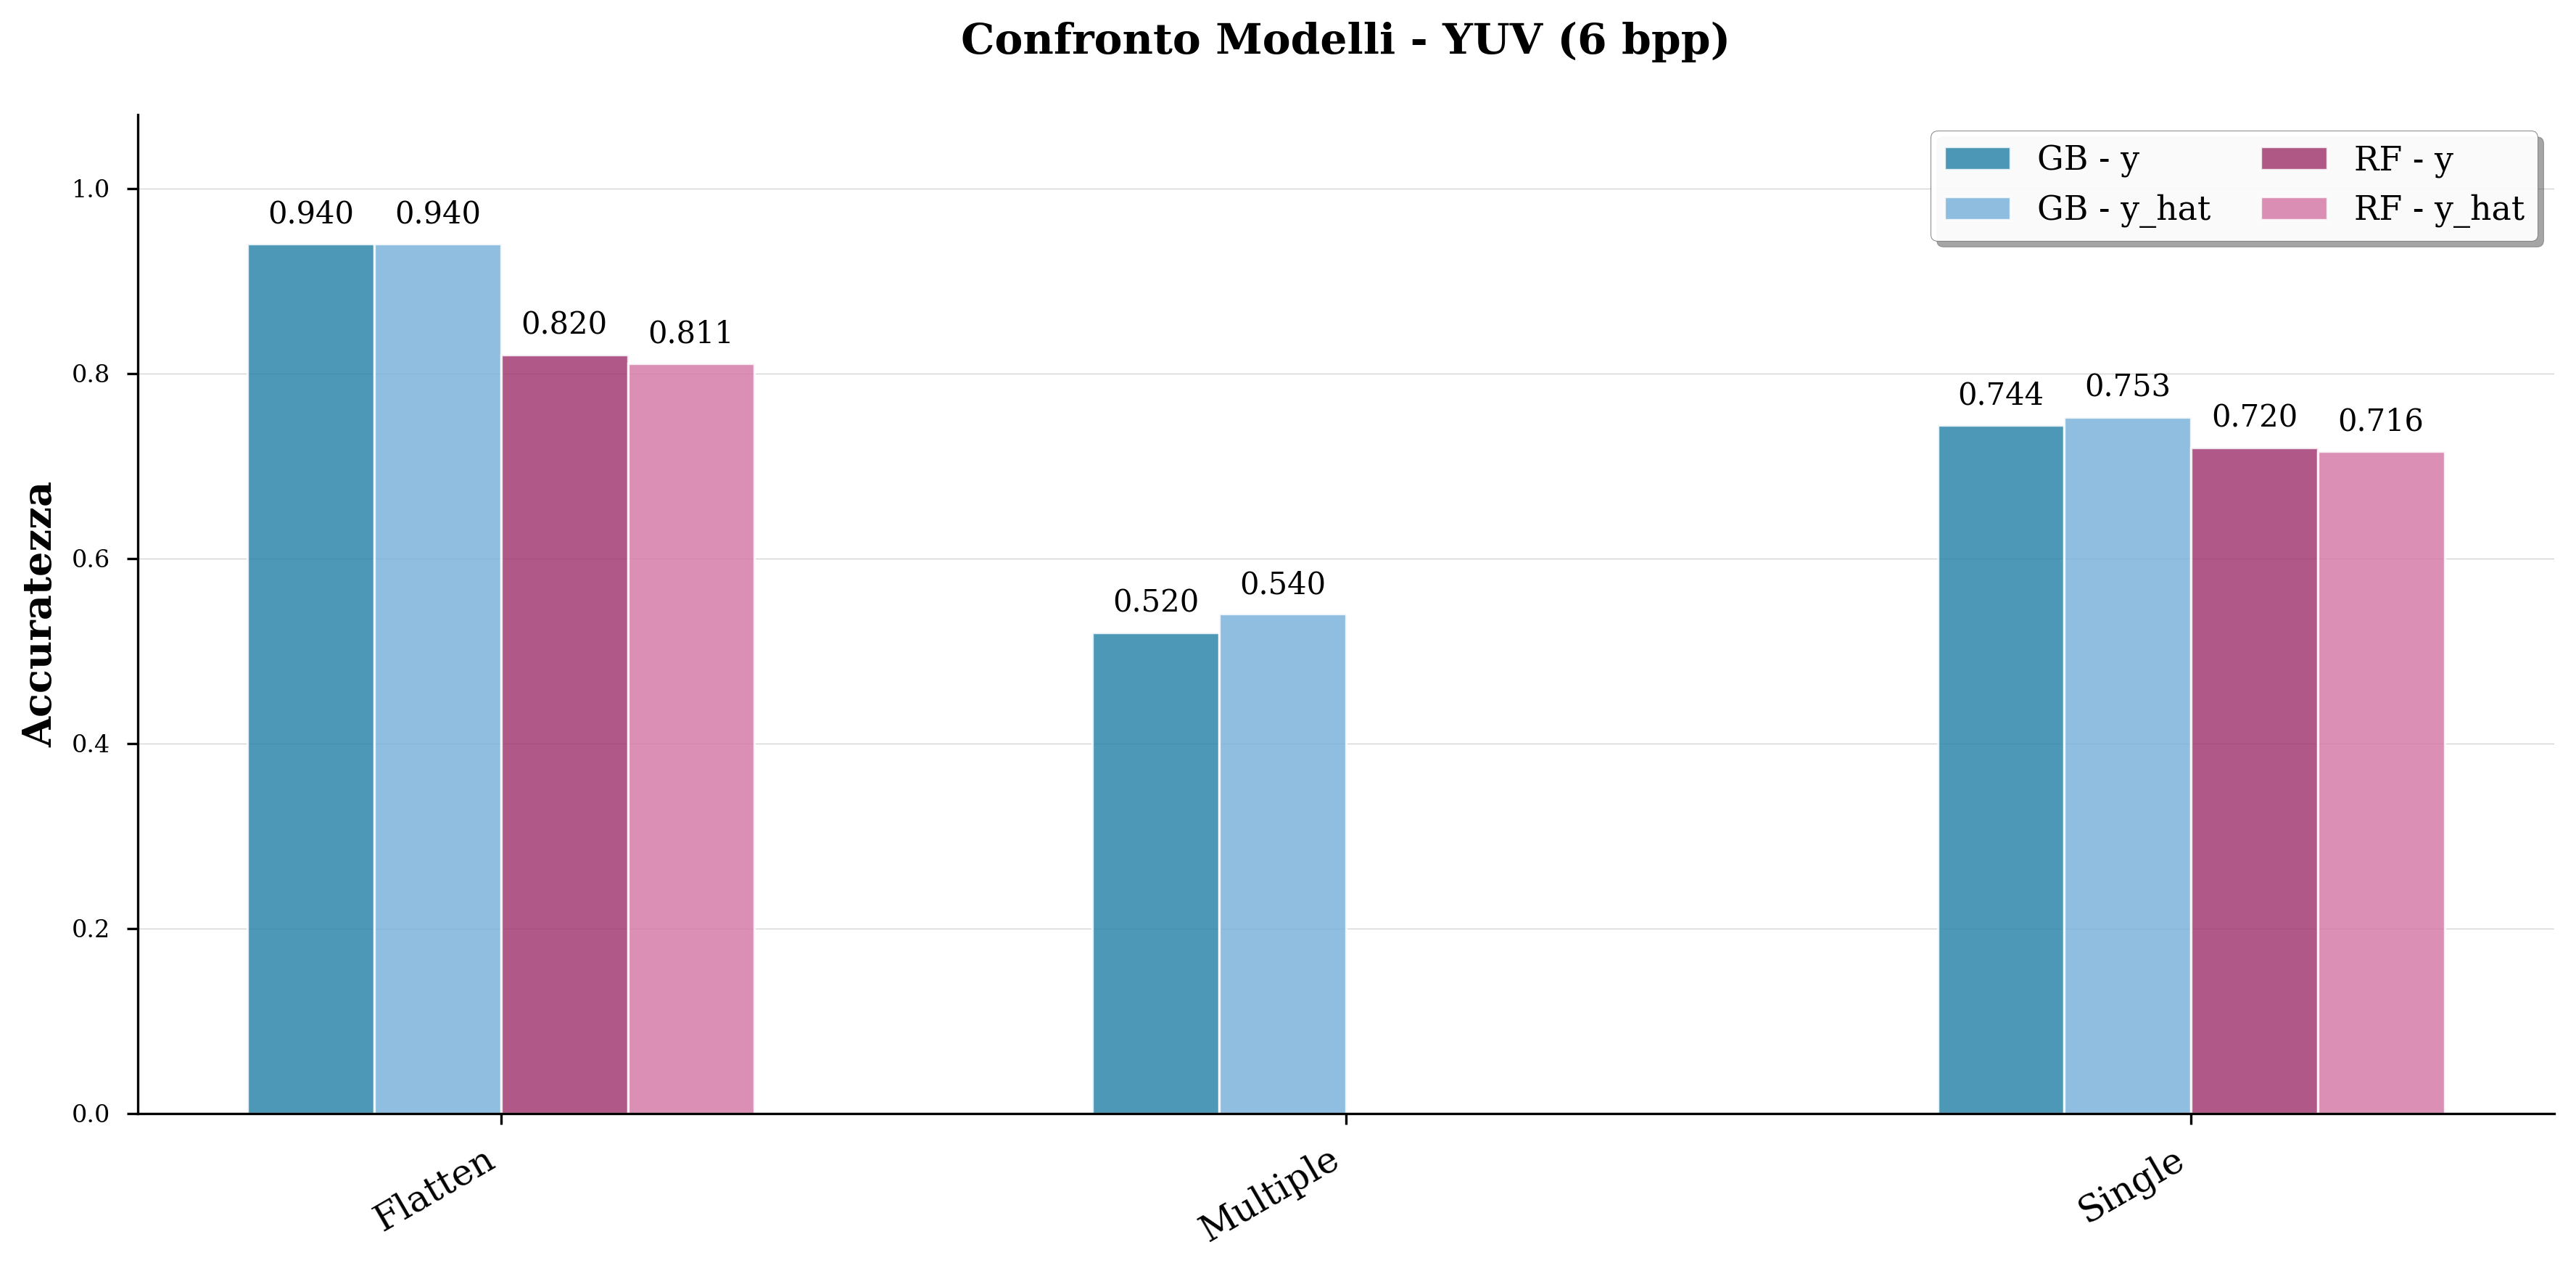
\includegraphics[width=\textwidth]{figures/Compare_GB_RF_YUV_6bpp_improved.png}
    \caption{Confronto tra Gradient Boosting e Random Forest a 6bpp.}
    \label{fig:GB_RF_Y_comparison}
\end{figure}

\begin{figure}
    \centering
    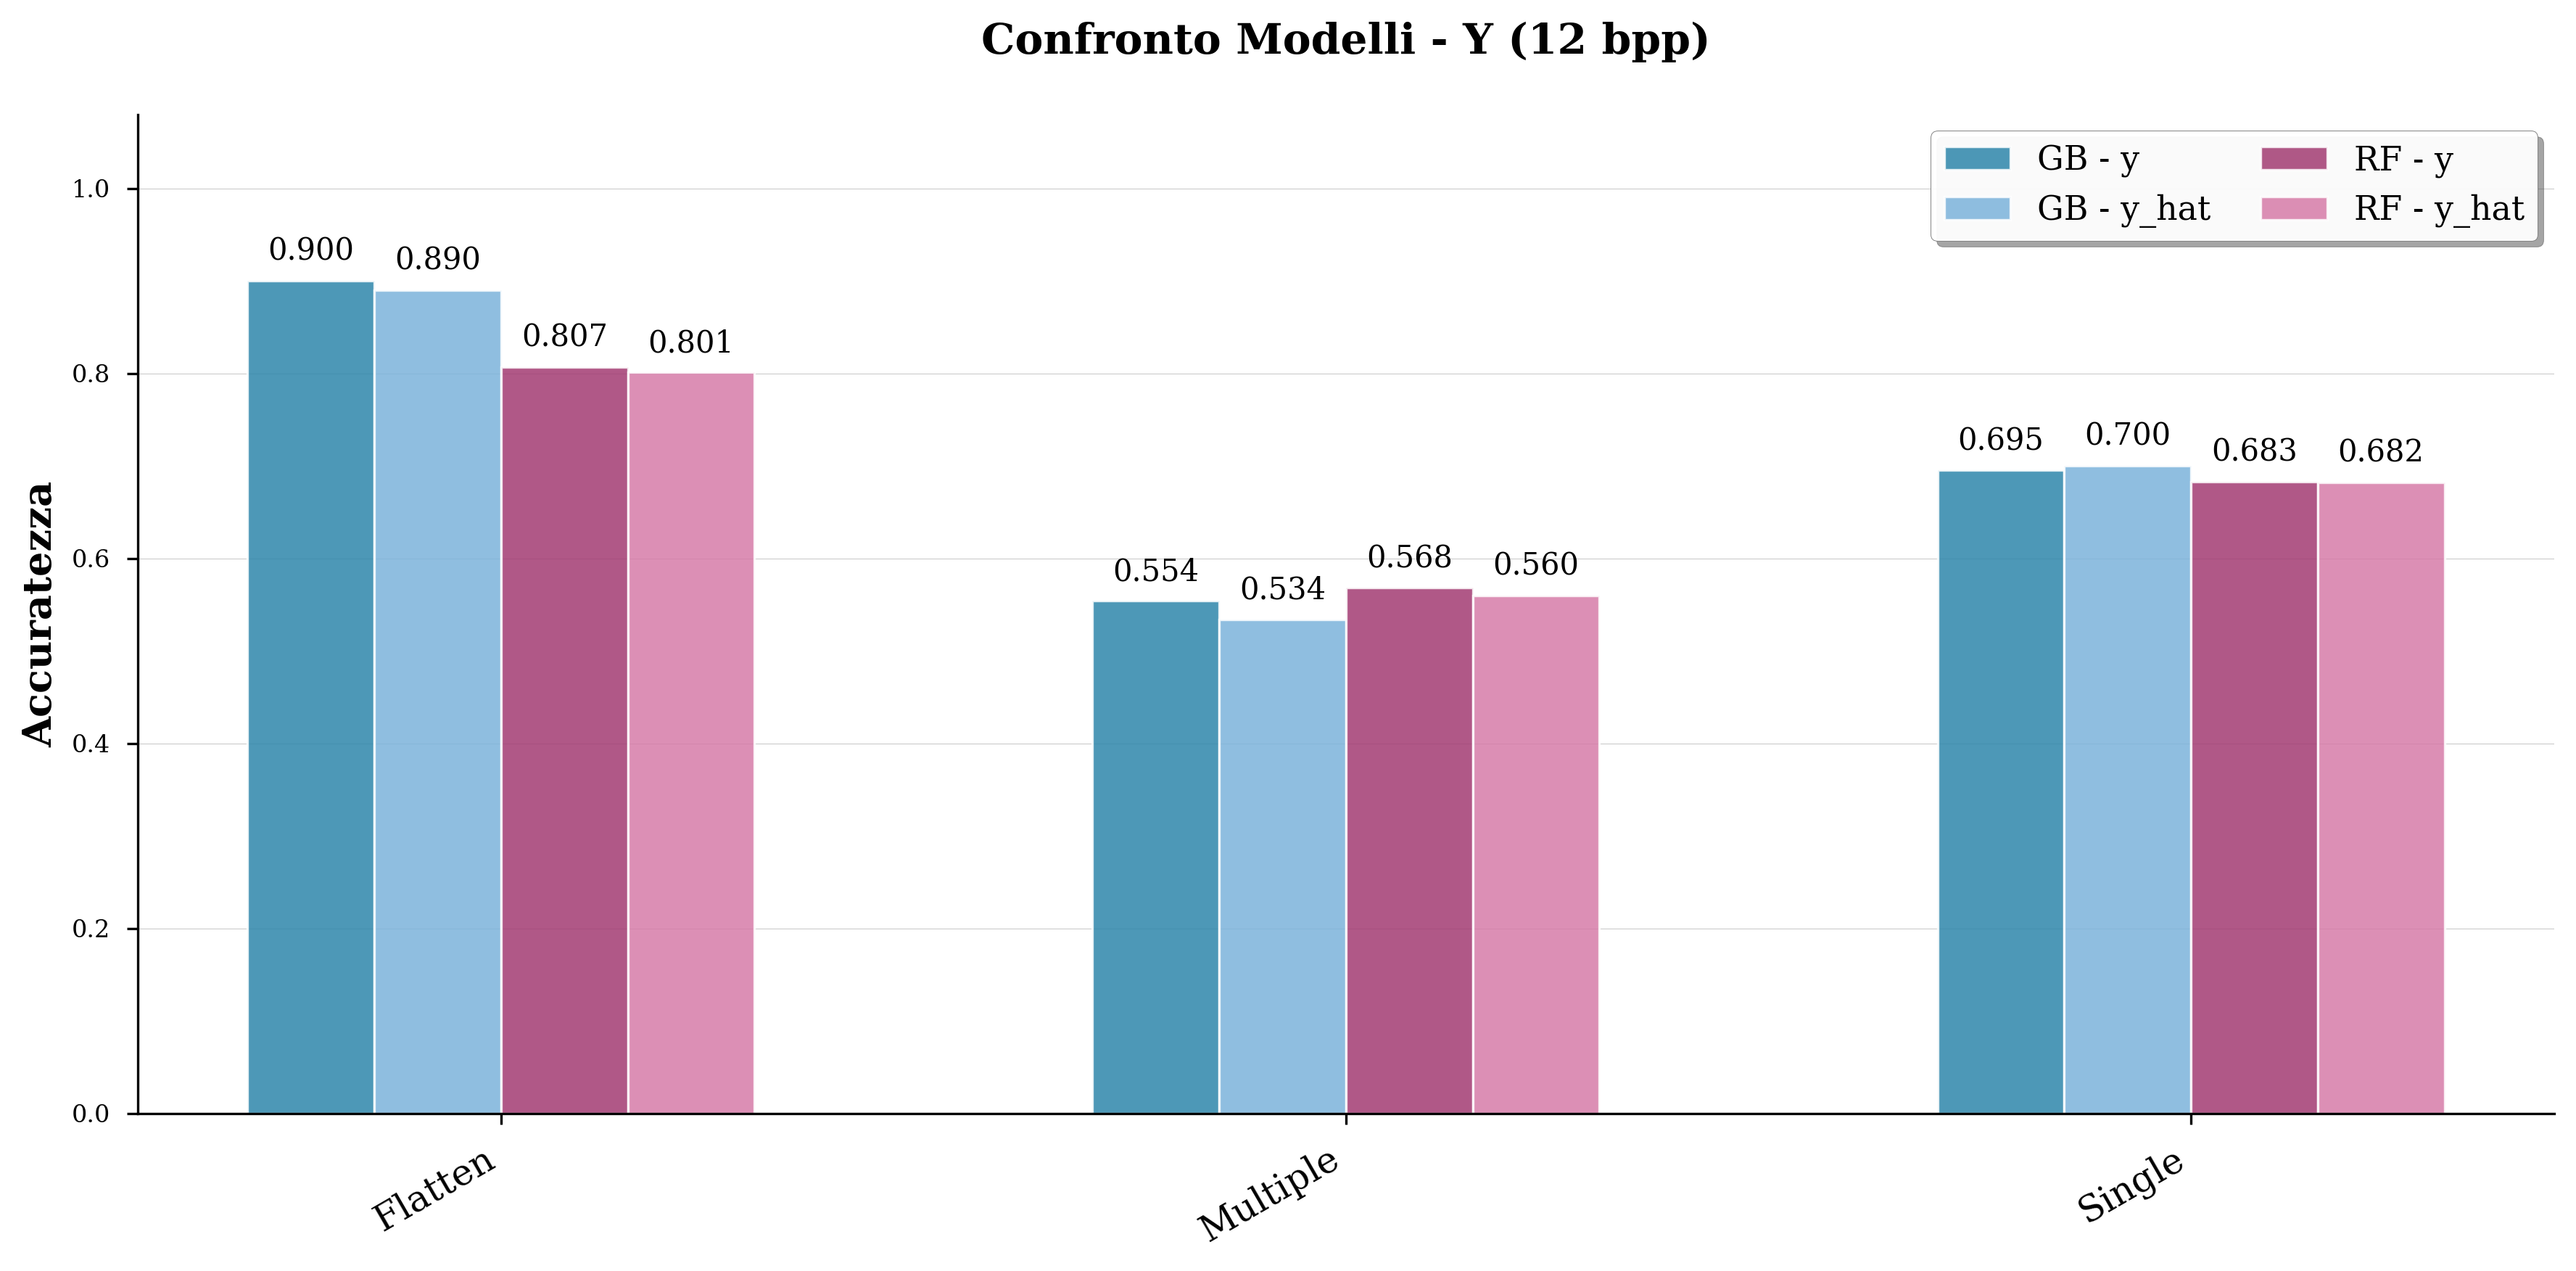
\includegraphics[width=\textwidth]{figures/Compare_GB_RF_Y_12bpp_improved.png}
    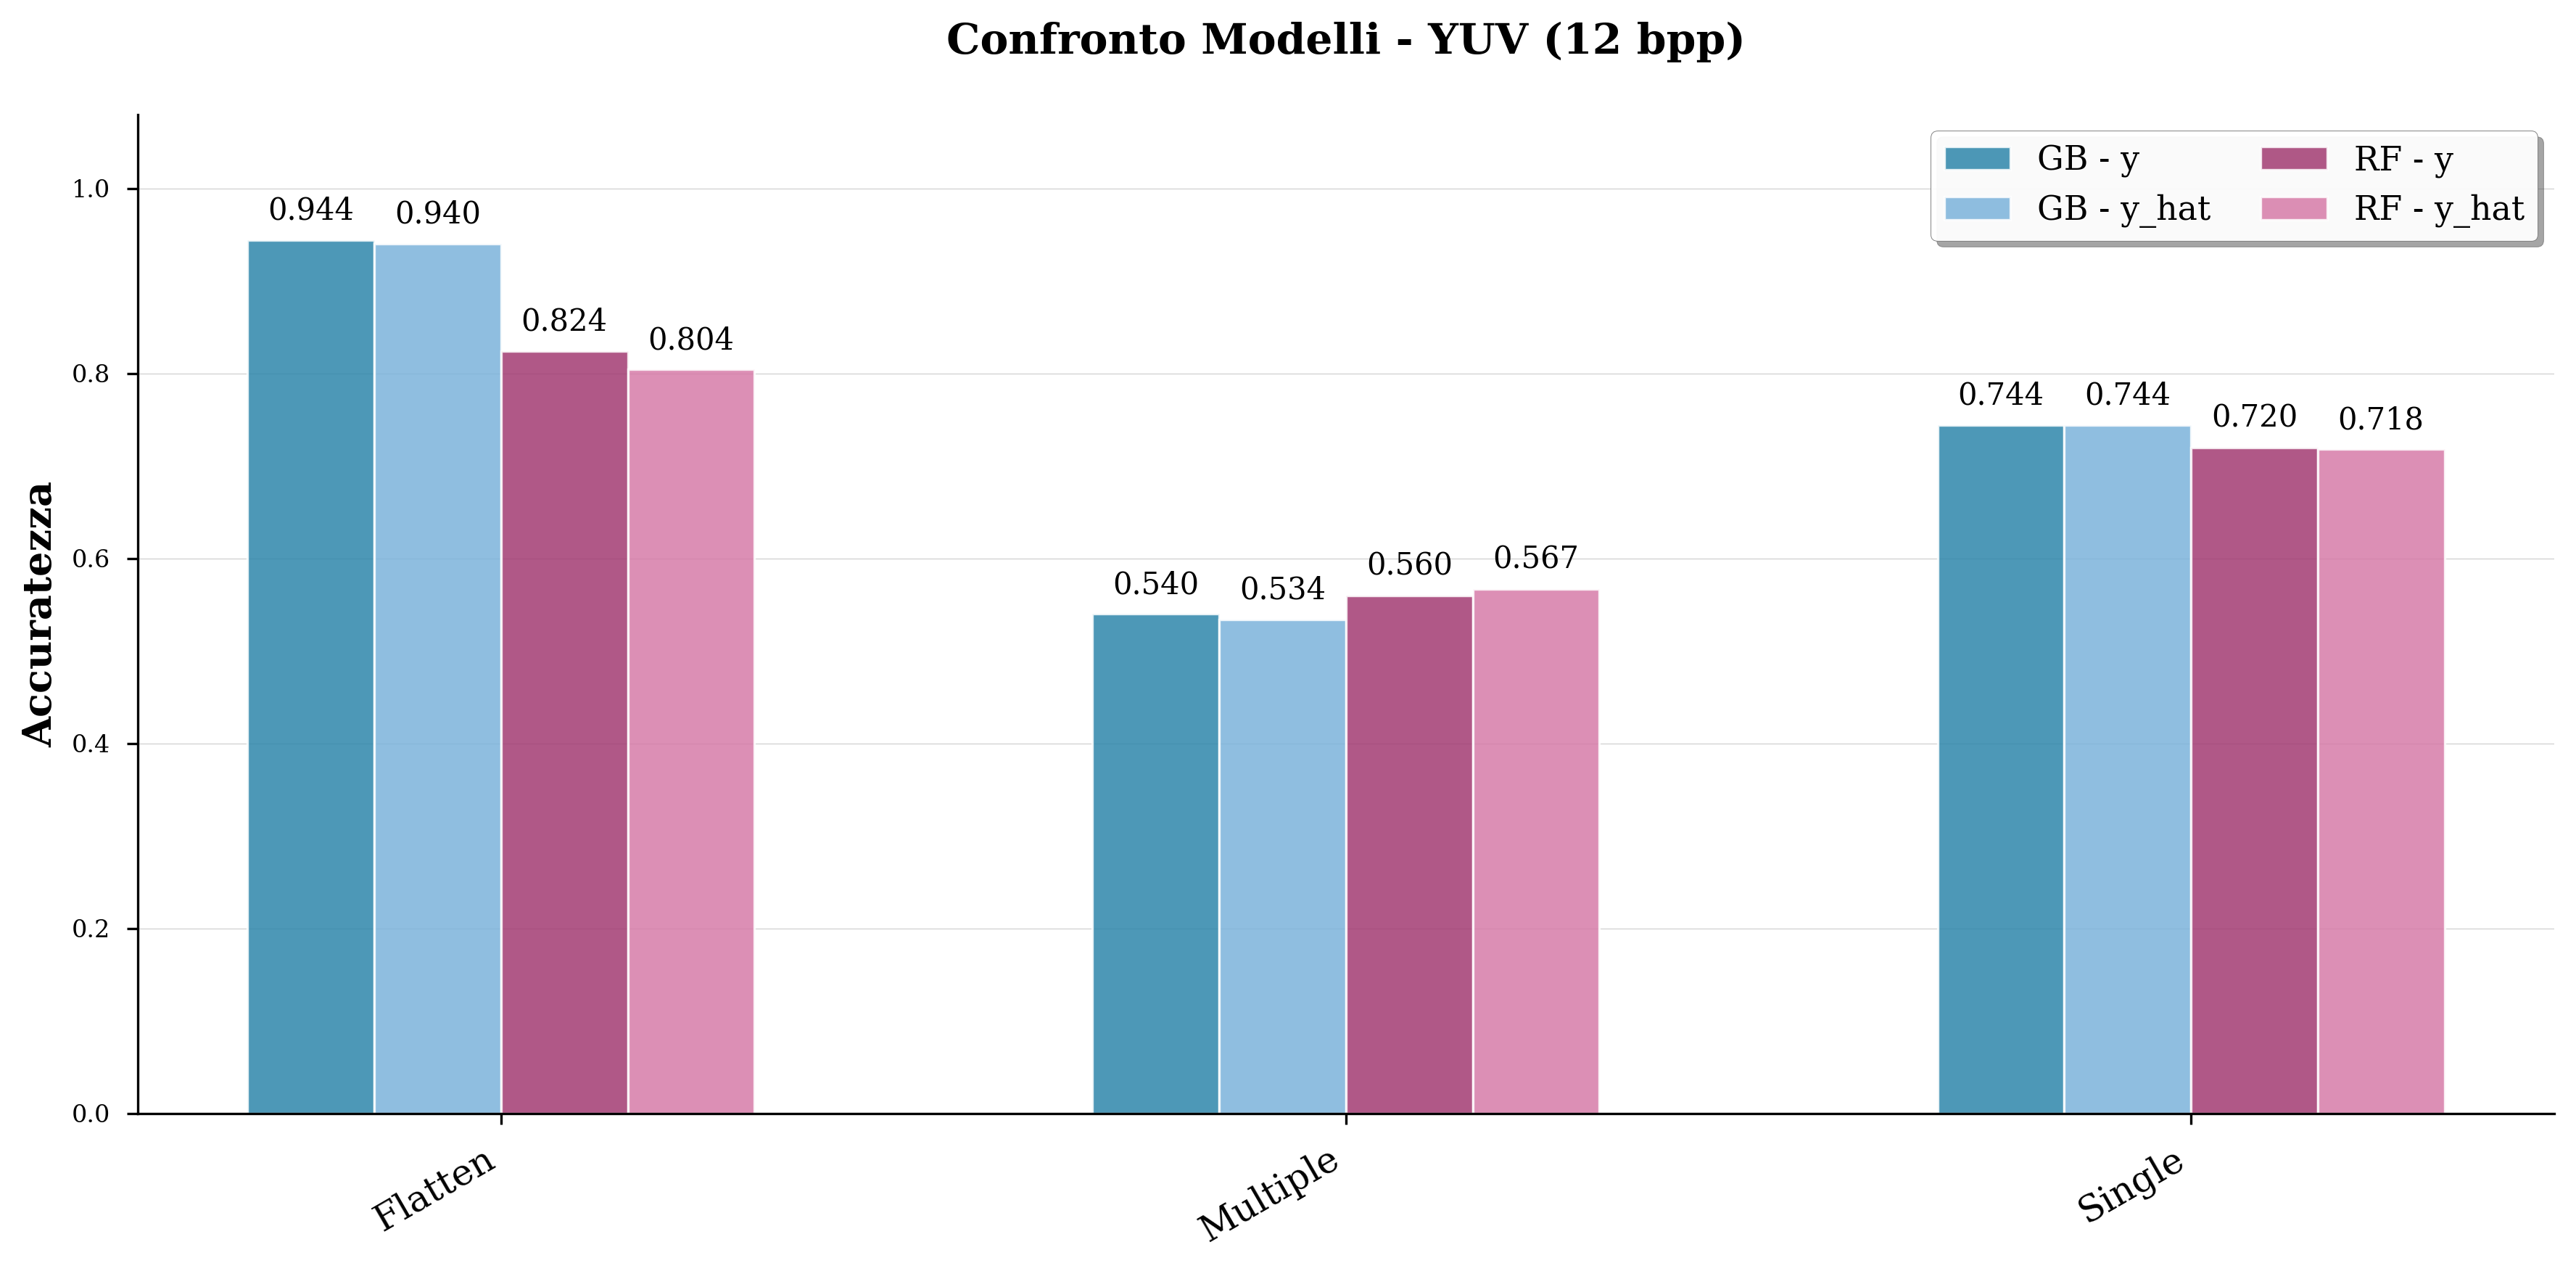
\includegraphics[width=\textwidth]{figures/Compare_GB_RF_YUV_12bpp_improved.png}
    \caption{Confronto tra Gradient Boosting e Random Forest a 12 bpp.}
    \label{fig:GB_RF_YUV_comparison}
\end{figure}
Dai diagrammi si può notare come l'accuratezza non subisca grandi varianzioni ai diversi livelli di compressione scelti, mentre è evidente la differenza tra le performance dei modelli allenati esclusivamente sulla componente di luminanza e quelli allenati anche usando la crominanza. Questo è ragionevole in quanto la differenza risiede nel fatto che nel secondo caso il classificatore ha più informazioni a disposizione da sfruttare nella classificazione. In tutti i casi però i modelli allenati solo sulla componente hanno avuto buoni risultati, ma la differenza delle prestazioni nel caso di tutte le componenti indica che buona parte dell'informazione che permette di discriminare immagini autentiche da quelle sintetiche risieda nelle componenti di crominanza.\\

Prestazioni diverse sono anche presenti nei diversi metodi di preprocessing delle feature. La miglior accuratezza in tutti casi è stata ottenuta dall'utilizzo del metodo di flattening, motivato dal fatto che questa tecnica non scarta nessuna informazione contenuta nelle rappresentazioni latenti originali. Questo incremento nelle prestazioni non avviene senza costi, infatti con l'aumento della dimensionalità dei campioni di esempio per addestrare i modelli, riportati nella tabella \ref{tab:preprocessing_methods}, corrisponde un aumento nei tempi di addestramento e una maggior necessità di risorse computazionali. Nella tabella \ref{tab:training_times} sono riportati i tempi di addestramento per ogni combinazione di fattori.
\begin{table}[H]
\centering
\caption{Tempi di addestramento su componenti YUV per dataset di $30.000$ immagini}\label{tab:training_times}
\begin{tabular}{l c c}
\toprule
Modello & Preprocessing & Tempo di addestramento \\
\midrule
RF &      single &  $\sim$3min \\
RF &    multiple &  $\sim$20min\\
RF &      flatten &  $\sim$1h45min\\
\midrule
GB &      single &  $\sim$2min \\
GB &    multiple &  $\sim$15min \\
GB &      flatten &  $\sim$1h \\
\bottomrule
\end{tabular}
\end{table}
Il metodo di single patch risulta essere il miglior compromesso tra accuratezza e tempi di addestramento, ma presenta il problema della forte dipendenza dalla posizione della patch estratta.\\
Il metodo multiple patches ha ottenuto risultati peggiori, ma ha la proprietà vantaggiosa di consentire di aumentare la cardinalità del dataset in casi dove non sono disponibili abbastanza campioni di addestramento, come mostrato nella tabella \ref{tab:preprocessing_methods}.\\

Le prestazioni simili ottenute con l'utilizzo di rappresentazioni quantizzate e non quantizzate indicano che il processo di quantizzazione interno al framework di JPEG AI riesce a conservare e non scartare eccessivamente le informazioni rilevanti.

Infine, osservando le tabelle \ref{fig:GB_RF_Y_comparison} e \ref{fig:GB_RF_YUV_comparison} si può notare come Gradient Boosting ottenga un'accuratezza in generale più alta rispetto a Random Forest, dovuta dalla diversa modalità con il quale vengono costruiti gli alberi di decisione di base.\\